% !Mode:: "Tex:UTF-8"

Los tres capítulos previos han establecido el lenguaje y los temas centrales de la Inferencia
clásica para una población. En este capítulo, vamos a ver cómo extender ese enfoque a otras
situaciones, que tienen como tema común su relación con la distribución binomial.

\section{Proporciones y su distribución muestral.}
\label{cap08:sec:ProporcionesDistribucionMuestral}

En una variable cuantitativa, como las que han centrado nuestra atención en los últimos capítulos,
la estimación de la media es la tarea más destacada. Pero si trabajamos con  una variable
cuantitativa, en la que la única información numérica relevante suele venir en forma de
frecuencias, entonces el parámetro interesante ya no es la media (que, de hecho, a menudo deja de
tener sentido). En estos casos, lo que nos interesa, la mayor parte de las veces, es conocer la
{\sf proporción} de elementos de la población que presentan una determinada característica.
Ejemplos típicos de esta clase de preguntas son:
\begin{itemize}
  \item ¿Qué {\em porcentaje} de españoles fuman?
  \item Después de un cruce de guisantes verdes con guisantes amarillos, ¿qué porcentaje de
      guisantes amarillos se da en su descendencia?
  \item ¿Cuál es la {\em tasa de supervivencia} a los cinco años, de los pacientes que han
      recibido cierto tratamiento?
  \item ¿Qué {\em fracción} de piezas defectuosas produce una máquina?
\end{itemize}

Lo que tienen en común todos estos ejemplos, es que tenemos una población $\Omega$, y que en los
individuos (o elementos) de esa población hay definida cierta característica que puede estar
presente o no en esos individuos (fumar/no fumar, sobrevivir/no sobrevivir, ser defectuosa/no
serlo).  Y en todos los casos, el parámetro que nos interesa es la {\sf proporción} $p$ de
individuos que poseen esa característica:
    \[p=\dfrac{\mbox{(número de individuos de la población con esa característica)}}{
    \mbox{(número total de individuos de la población, con o sin esa característica)}}.\]

Al igual que hemos hecho en anteriores capítulos, vamos a utilizar un ejemplo concreto como hilo
conductor de nuestro trabajo sobre proporciones.
\begin{ejemplo}\label{cap08:ejem:Araos}

Por ejemplo, podemos fijarnos en la población de Araos Comunes ({\em Uria aalge}, en inglés {\em Common
Guillemot}), una especie de aves marinas, común en el Atlántico Norte. Puedes ver más información
sobre ellos en el enlace [\,\ref{enlace0016}\,]\label{enlace0016a}, de la  Wikipedia. Esta especie presenta un polimorfismo en su plumaje, que consiste en la existencia, en algunos ejemplares de un anillo ocular blanco (estos ejemplares se denominan {\em embridados}; {\em bridled}, en inglés). La Figura \ref{cap07:fig:Araos} muestra una imagen de una colonia de cría en Escocia. Puede verse en el centro uno de estos ejemplares embridados rodeado de ejemplares sin esa característica.

\begin{figure}[htbp]
\begin{center}
\begin{enColor}

\includegraphics[width=13cm]{../fig/Cap08-araos.png}
\end{enColor}
\begin{bn}
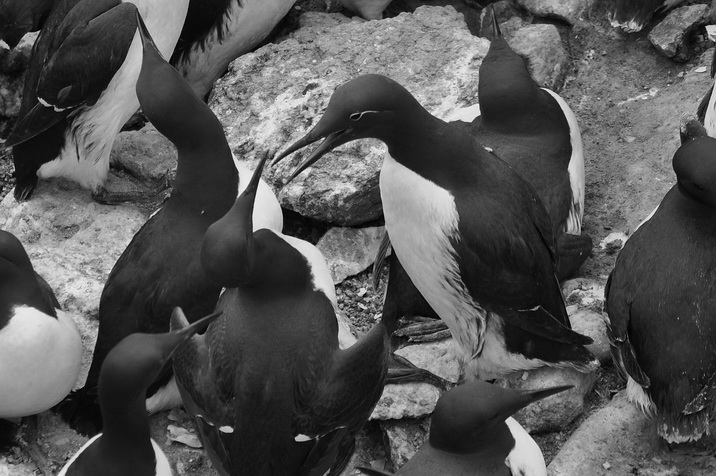
\includegraphics[width=13cm]{../fig/Cap08-araos-bn.png}
\end{bn}
\caption{Araos comunes en la isla Lunga, en las Thresnish, Escocia.}
\label{cap07:fig:Araos}
\end{center}
\end{figure}

Una pregunta natural es ¿cuál es la proporción de ejemplares embridados sobre el total de individuos de la especie? Para responderla, como siempre, tenemos que acudir a una muestra. En un artículo de 2010 (ver referencia \cite{reiertsen2012climate}), Reiersten et al. incluyen la Tabla \ref{cap08:tabla:PaperFrecuenciaAraosEmbridados}, con los resultados de distintas muestras, tomadas a lo largo de una serie de años en la isla noruega de Horn{\o}ya.

    \begin{table}[htb]
    \begin{center}
    \begin{tabular}{cccc}
        Año&Embridados&No-embridados&\% aves embridadas\\
        1989&39&66&37.1\\
        2005&75&138&35.2\\
        2008&86&180&32.3\\
        2009&138&270&33.8\\
        2010&139&317&30.5
    \end{tabular}
    \caption{Frecuencias de araos embridados y no embridados, datos de \cite{reiertsen2012climate}, Tabla 2.}
    \label{cap08:tabla:PaperFrecuenciaAraosEmbridados}
    \end{center}
    \end{table}
    Como puede verse, los autores calculan el porcentaje de aves embridadas a partir de las muestras. ¿Podemos usar esos porcentajes para construir intervalos de confianza para la proporción en la población, para esos años?
\qed
\end{ejemplo}

Vamos a fijar la terminología necesaria para responder a preguntas como esta. Ya hemos dicho que
vamos a llamar $p$ a la proporción de individuos de la especie que presentan la característica que
es objeto de estudio. ¿Qué tipo de variables aleatorias intervienen en este problema? Cada
individuo puede tener, o no, la característica que nos interesa, y la probabilidad de que un
individuo, elegido al azar, la tenga, es precisamente la proporción $p$. Así que parece que tenemos
una de esas situaciones de sí/no que, en el Capítulo \ref{cap:TeoremaCentralLimite} (pág.
\pageref{cap05:def:ExperimentoBernouilli}) llamábamos un {\em Experimento de Bernouilli}. Por
tanto, la variable aleatoria
\[X=\{\mbox{el individuo presenta esa característica}\}\]
es de tipo Bernouilli$(p)$. Dicho de otra forma, es una binomial $B(1,p)$. Su media es
$\mu_X=1\cdot p=p$ y su desviación típica es $\sigma_X=\sqrt{1\cdot p\cdot q}=\sqrt{p\cdot q}$.

Para estimar el valor de $p$, tomamos una muestra aleatoria de la población, formada por $n$
observaciones. Recordemos que eso significa que tenemos $n$ variables aleatorias independientes,
    \[X_1,X_2,\ldots,X_n\]
y que la distribución de probabilidad para cada una de ellas es una copia de la distribución de
probabilidad de la población original.

¿Cómo usamos la muestra para estimar $p$? Pues contamos el número de individuos de la muestra que
presentan esa característica, y dividimos entre el número $n$ de elementos de la muestra. El número
resultante es lo que vamos a llamar la {\sf proporción muestral:}\index{proporción muestral}
    \begin{equation}\label{cap08:ecu:ProporcionMuestral}
        \hat p=\dfrac{X_1+X_2+\cdots+X_n}{n}
    \end{equation}
para distinguirlo de $p$, al que si es preciso llamaremos {\sf proporción
poblacional}\index{proporción poblacional}.

Por lo tanto, la proporción muestral es simplemente la media de una lista de variables
independientes de tipo $B(1,p)$. Fijándonos en el numerador, ¿qué se obtiene  al sumar $n$
variables independientes de tipo $B(1,p)$? Pues, pensándolo un poco, nos daremos cuenta de que se
obtiene una binomial $B(n,p)$. Por lo tanto la variable proporción muestral $\hat p$ es una
binomial $B(n,p)$ {\em pero dividida por $n$}. Esto lo representamos así:
    \[\hat p \sim \colorbox{lightgrey}{${\dfrac{1}{n}}$}B(n,p).\]
Ahora necesitamos recordar los resultados de las Ecuaciones \ref{cap05:ecu:MediaBinomial} y
\ref{cap05:ecu:DesviaciontipicaBinomial} (pág. \pageref{cap05:ecu:MediaBinomial}) para la binomial,
y los de la página \pageref{cap04:lugar:OperacionesVariablesAleatorias} sobre operaciones con
variables aleatorias. Usando esta información, obtenemos, para la media:
    \[E\left(\dfrac{1}{n}B(n,p)\right)=\dfrac{1}{n}\cdot E(B(n,p))=\dfrac{n\cdot p}{n}=p,\]
Mientras que para la varianza es:
    \[\operatorname{Var}\left(\dfrac{1}{n}B(n,p)\right)=\left(\dfrac{1}{n}\right)^2\cdot \operatorname{Var}(B(n,p))=\dfrac{n\cdot p\cdot q}{n^2}=\dfrac{p\cdot q}{n}.\]
Por lo tanto, hemos obtenido este resultado:

    \begin{center}
    \fcolorbox{black}{Gris025}{
    \begin{minipage}{12.5cm}
        %%%%%%%%%%%%%%%%%%%%%%%%%%%%%%%%%%%%%%%
        \begin{center}
        {\bf Distribución de la proporción muestral $\hat p$.}
        \index{proporción muestral, distribución}
        \end{center}
       %%%%%%%%%%%%%%%%%%%%%%%%%%%%%%%%%%%%%%%
            Sea $X$ una variable aleatoria de tipo $B(1,p)$, y sea $(X_1,X_2,\ldots,X_n)$ una muestra aleatoria independiente de tamaño $n$ de $X$. Si llamamos
                \[\hat p=\dfrac{X_1+X_2+\cdots+X_n}{n}\]
            entonces
                \begin{equation}\label{cap08:ecu:ProporcionMuestralEsBinomial}
                    \hat p \sim \dfrac{1}{n}B(n,p)
                \end{equation}
            y por lo tanto:
               \[\mu_{\hat p}=p, \qquad \sigma_{\hat p}=\sqrt{\dfrac{p\cdot q}{n}}.\]
       %%%%%%%%%%%%%%%%%%%%%%%%%%%%%%%%%%%%%%%
    \end{minipage}}
    \end{center}
Vamos a utilizar esta información para construir un intervalo de confianza para la proporción.

\subsection{Intervalo de confianza para la proporción.}
\label{cap08:sec:IntervaloConfianzaProporcion}

El siguiente paso, siguiendo las pautas que establecimos en el Capítulo
\ref{cap:IntervalosConfianza}, es encontrar un estadístico que podamos utilizar para estimar $p$ a
partir de una muestra. El punto de partida es la Ecuación \ref{cap08:ecu:ProporcionMuestralEsBinomial}
que hemos descubierto. Podríamos trabajar directamente a partir de aquí, pero eso nos llevaría a
depender de la binomial. En los últimos años, con la facilidad para el cálculo que han aportado los
ordenadores, ese tipo de métodos han recibido un interés renovado. Pero, para empezar, vamos a
mantenernos en el terreno de los métodos clásicos, y vamos a buscarle un sustituto a la Binomial.
Ya sabemos, por nuestro trabajo del Capítulo \ref{cap:TeoremaCentralLimite} (ver, especialmente el
Teorema Central del Límite, pág. \pageref{cap05:teo:TCL}), que podemos usar la Normal, siempre que
se cumplan algunas condiciones. En concreto, debe ser:
\begin{equation}\label{cap08:ecu:condicionesTCLPrimeraVersion}
    n\cdot p> 5,\mbox{ y a la vez }n\cdot q>5.
\end{equation}
(Recuerda que $q=1-p$). Nuestros adversarios, por tanto, para poder hacer esto son dos:
\begin{itemize}
  \item Las muestras muy pequeñas.
  \item Los casos en los que $p$ (o $q$) es muy pequeño.
\end{itemize}
En la segunda parte de este capítulo nos vamos a ocupar especialmente del caso en el que $p$ es muy
pequeño. De momento, en el resto de esta sección, {\em vamos a trabajar asumiendo que se cumplen
las condiciones \ref{cap08:ecu:condicionesTCLPrimeraVersion}}. En ese caso, estamos bajo el
paraguas del Teorema Central del Límite, y la tarea de definir el Estadístico adecuado se
simplifica considerablemente. Usando ese teorema en la Ecuación \ref{cap08:ecu:ProporcionMuestralEsBinomial}, se obtiene una aproximación normal a la distribución muestral de $\hat p$:
    \begin{equation}
    \label{cap08:ecu:DistribucionMuestralProporcionAproximacionNormal}
        \hat p \sim \dfrac{1}{n}B(n,p)
        \sim \dfrac{1}{n}N(n\cdot p,\sqrt{n\cdot p\cdot q}=
        N\left(\dfrac{n\cdot p}{n},\dfrac{\sqrt{n\cdot p\cdot q}}{n}\right)=
        N\left(p,\sqrt{\dfrac{p\cdot q}{n}}\right)
    \end{equation}
Para obtener un estadístico útil a partir de esto, sólo nos queda un pequeño problema, similar al que ya tuvimos en su momento en el caso de la media. La desviación típica de la aproximación normal a $\hat p$ es, según la Ecuación \ref{cap08:ecu:DistribucionMuestralProporcionAproximacionNormal}:
    \[\sqrt{\dfrac{p\cdot q}{n}},\]
pero no podemos usar esto directamente, porque desconocemos el valor de $p$. Así que lo que vamos a
hacer es reemplazarlo con
    \[\sqrt{\dfrac{\hat p\cdot \hat q}{n}},\]
(donde $\hat q=1-\hat p$), que es el valor que podemos calcular a partir de la muestra. Para que
esa sustitución funcione, debemos asegurarnos de utilizar muestras grandes. Poniendo todas las
piezas juntas, tenemos el estadístico que necesitamos.
    \begin{center}
    \fcolorbox{black}{Gris025}{
    \begin{minipage}{12.5cm}
        %%%%%%%%%%%%%%%%%%%%%%%%%%%%%%%%%%%%%%%
        \begin{center}
        {\bf Estadístico para proporciones.}
        \end{center}
       %%%%%%%%%%%%%%%%%%%%%%%%%%%%%%%%%%%%%%%
       Sea $X$ una variable aleatoria de tipo $B(1,p)$. Tomamos muestras independientes de $X$ de tamaño $n$, y suponemos que se cumplen, a la vez estas condiciones:
       \[n>30,\quad n\cdot\hat p>5,\quad n\cdot\hat q>5,\]
       Entonces, a medida que consideramos muestras de tamaño $n$ cada vez más grande, la distribución de la proporción muestral $\hat p$ se aproxima cada vez más a la normal
            \begin{equation}
            \label{cap08:ecu:DistribucionMuestralProporcionAproximacionNormal02}
            N\left(p,\sqrt{\dfrac{\hat p\cdot\hat q}{n}}\right).
            \end{equation}
       En particular, para las condiciones dadas, tenemos este {\sf estadístico para proporciones}\index{estadístico para proporciones}:
       \begin{equation}\label{cap08:ecu:EstadisticoProporciones}
        Z=\dfrac{\hat p-p}{\sqrt{\dfrac{\hat p\cdot \hat q}{n}}}\sim N(0,1).
       \end{equation}
       cuya distribución, como se indica, es la normal estándar $Z$.\\
       %%%%%%%%%%%%%%%%%%%%%%%%%%%%%%%%%%%%%%%
    \end{minipage}}
    \end{center}
Ya hemos visto, en el Capítulo \ref{cap:IntervalosConfianza}, que la información sobre la
distribución del estadístico es todo lo que se necesita. No nos vamos a demorar más en obtener el
intervalo de confianza, porque el razonamiento es idéntico a otros que ya hemos hecho. El resultado
es este:
    \begin{center}
    \fcolorbox{black}{Gris025}{
    \begin{minipage}{13.2cm}
        %%%%%%%%%%%%%%%%%%%%%%%%%%%%%%%%%%%%%%%
				\begin{center}
        {\bf Intervalo de confianza (nivel $(1-\alpha$)) para la proporción $p$, muestra grande}
        \index{intervalo de confianza para la proporción $p$, muestra grande}
				\end{center}
       %%%%%%%%%%%%%%%%%%%%%%%%%%%%%%%%%%%%%%%
       Si se cumplen, a la vez:
       \[n>30,\quad n\cdot\hat p>5,\quad n\cdot\hat q>5.\]
       entonces el intervalo de confianza al nivel $(1-\alpha)$  para la proporción $p$ es:
       \begin{equation}\label{cap08:ecu:IntervaloConfianzaProporcionMuestraGrande}
        \hat p-z_{\alpha/2}\sqrt{\dfrac{\hat p\cdot \hat q}{n}}\leq p \leq \hat p +z_{\alpha/2}\sqrt{\dfrac{\hat p\cdot \hat q}{n}}.
       \end{equation}
       que también escribiremos a veces:
       \[p =\hat p \pm z_{\alpha/2}\sqrt{\dfrac{\hat p\cdot \hat q}{n}}.\]
       %%%%%%%%%%%%%%%%%%%%%%%%%%%%%%%%%%%%%%%
    \end{minipage}}
    \end{center}

Veamos en un ejemplo el problema de los araos embridados que hemos descrito al principio de este
capítulo.
\begin{ejemplo}\label{cap08:ejem:IntervaloConfianzaProporcionAraos}
Vamos a calcular un intervalo de confianza, al 95\%, para la proporción de araos embridados del año
2010. Ese año se contabilizaron (ver la Tabla \ref{cap08:tabla:PaperFrecuenciaAraosEmbridados},
pág. \pageref{cap08:tabla:PaperFrecuenciaAraosEmbridados}) 139 araos embridados y 317 no
embridados, así que la muestra es grande, de $n=139+317=456$ individuos. Además las proporciones
muestrales de embridados y no embridados son, respectivamente:
\[\hat p=\dfrac{139}{456}\approx 0.3048,\quad\mbox{y}\quad\hat q=\dfrac{317}{456}\approx 0.6952\]
Fíjate que en casos como este,
\[n\cdot \hat p=139,\quad n\cdot \hat q=317 \]
así que para cumplir las condiciones, basta con saber que la muestra es de más de 30 individuos y
que hay al menos 5 de cada clase.

Como en otros casos, tenemos $\alpha=0.05$, y calculamos $z_{\alpha/2}=z_{0.025}\approx 1.960$, así
que, sustituyendo en la Ecuación \ref{cap08:ecu:IntervaloConfianzaProporcionMuestraGrande} del
intervalo se obtiene:
    \[
    \hat p \pm z_{\alpha/2}\sqrt{\dfrac{\hat p\cdot \hat q}{n}}=
    \dfrac{139}{456}\pm 1.960\sqrt{\dfrac{\left(\dfrac{139}{456}\right)\cdot\left(\dfrac{317}{456}\right)}{456}}
    \approx \dfrac{139}{456}\pm 0.04225.
    \]
Es decir que el intervalo es: $(0.2626,0.3471)$. \qed
\end{ejemplo}


\subsection{Contraste de hipótesis para la proporción.}
\label{cap08:subsec:ContrasteHipotesisProporcion}

A riesgo de ser reiterativos: una vez que se conoce el estadístico adecuado, y su distribución,
tanto los intervalos de confianza (que ya hemos visto) como los contrastes de hipótesis, son muy
fáciles de obtener. Como en los intervalos de confianza, suponemos que se cumplen, a la vez:
       \[n>30,\quad n\cdot\hat p>5,\quad n\cdot\hat q>5.\]
Entonces, los contrastes, según el tipo de hipótesis nula, son estos {\em ({!`}atención a los
cuantiles $z_p$ utilizados en cada caso!)}:
\begin{enumerate}
    \item[] {\sf En todos los casos $q_0 = 1-p_0$}
    \item[(a)] Hipótesis nula: $H_0=\{p\leq p_0\}$.\\
        Región de rechazo:
        \[\hat p>p_0+z_{\alpha}\sqrt{\dfrac{p_0\cdot q_0}{n}}.\]
        \begin{equation}\label{cap08:ecu:pValorProporcionColaDerecha}
        \mbox{p-valor}=
        P\left(Z > \dfrac{\hat p-p_0}{\sqrt{\dfrac{p_0\cdot q_0}{n}}}\right)
        \end{equation}
    \item[(b)] Hipótesis nula: $H_0=\{p\geq p_0\}$.\\
        Región de rechazo:
        \[\hat p<p_0+z_{1-\alpha}\sqrt{\dfrac{p_0\cdot q_0}{n}}.\]
        \begin{equation}\label{cap08:ecu:pValorProporcionColaIzquierda}
        \mbox{p-valor}=
        P\left(Z < \dfrac{\hat p-p_0}{\sqrt{\dfrac{p_0\cdot q_0}{n}}}\right)
        \end{equation}
    \item[(c)] Hipótesis nula: $H_0=\{p=p_0\}$.\\
        Región de rechazo:
        \[|\hat p-p_0|>z_{\alpha/2}\sqrt{\dfrac{p_0\cdot q_0}{n}}.\]
        \begin{equation}\label{cap08:ecu:pValorProporcionBilateral}
        \mbox{p-valor}=\colorbox{lightgrey}{\large\bf 2}\cdot P\left(Z >
        \dfrac{\colorbox{lightgrey}{$|\hat p-p_0|$}}{\sqrt{\dfrac{p_0\cdot q_0}{n}}}\right)
        \end{equation}
        Para entender los dos aspectos que hemos destacado en este último caso (el 2 y el valor
        absoluto), conviene revisar la discusión que hicimos sobre la Ecuación
        \ref{cap07:ecu:pValorMediaZBilateral} (pág. \pageref{cap07:ecu:pValorMediaZBilateral}).
\end{enumerate}
En todos estos contrastes hay una diferencia sutil, pero importante, como en el caso de la media
que vimos en el Capítulo \ref{cap:ContrasteHipotesis}. Puesto que el contraste se basa en suponer
que la hipótesis nula es cierta, hemos utilizado $p_0$ y $q_0=1-p_0$ en lugar de $\hat p$ y $\hat
q$. La razón de hacer esto es que, como hemos dicho, si suponemos que la hipótesis nula es cierta,
entonces la desviación típica de la proporción muestral sería $\sqrt{\dfrac{p_0\cdot q_0}{n}}$. En
el caso de la media, sin embargo, suponer conocida la media $\mu_0$ de la población no nos servía
para saber cuál es la desviación típica de la población, y por eso usábamos $s$ como sustituto.

Vamos a ver un ejemplo, basado todavía en los datos de los araos embridados.
\begin{ejemplo}\label{cap08:ejem:ContrasteHipotesisProporcionAraos}
La Tabla \ref{cap08:tabla:PaperFrecuenciaAraosEmbridados} (pág.
\pageref{cap08:tabla:PaperFrecuenciaAraosEmbridados}) muestra que en el año 1989 se contabilizaron
39 araos embridados y 66 no embridados (es decir $n=39+66=105$). Un investigador sospecha que la
proporción de embridados, en ese año, era superior al 35\%. ¿Avalan estos datos su sospecha?

La hipótesis alternativa es $H_a=\{p>p_0\}$, y la nula es, por supuesto
\[ H_0=\{p\leq p_0\},\]
con $p_0=0.35$, así que estamos en el caso (a). Además las proporciones muestrales de embridados y
no embridados son, respectivamente:
\[\hat p=\dfrac{39}{105}\approx 0.3714,\quad\mbox{y}\quad\hat q=\dfrac{66}{105}\approx 0.6286\]
Para calcular el p-valor usamos la Ecuación \ref{cap08:ecu:pValorProporcionColaDerecha}
        \[
        \mbox{p-valor}=
        P\left(Z > \dfrac{\hat p-p_0}{\sqrt{\dfrac{p_0\cdot q_0}{n}}}\right)=
        P\left(Z > \dfrac{\dfrac{39}{105}-0.35}{\sqrt{\dfrac{0.35\cdot 0.65}{105}}}\right)=
        P\left(Z > 0.4604\right)\approx 0.3226
        \]
Observa que el valor del estadístico es aproximadamente 0.4604. Así que, con este p-valor, no
rechazamos la hipótesis nula, y el investigador no puede confirmar su sospecha basándose en estos
datos. \qed
\end{ejemplo}


\subsection{El método exacto de Clopper y Pearson.}
\label{cap08:subsec:MetodoExactoBinomial}
\noindent{\bf Opcional: esta sección puede omitirse en una primera lectura.}\\

En los apartados anteriores hemos usado la aproximación de la binomial por la normal para realizar
inferencia, tanto en el caso de los intervalos de confianza, como en el de los contrastes de
hipótesis. Pero debemos tener presente que hay casos en los que esa aproximación no es posible,
porque no se cumplen las condiciones necesarias. En particular, eso sucede cuando $p$ es muy
pequeño, caso que veremos en la Sección \ref{cap08:sec:DistribucionPoisson}, o cuando las muestras
son pequeñas.  Aquí vamos a fijarnos especialmente en el caso de muestras de tamaño pequeño.  Al
usar la normal para muestras de tamaño grande, lo que hemos estado haciendo es una {\em
aproximación} que, para tamaños muestrales pequeños, deja de ser válida. Por lo tanto, es posible preguntarse si, para trabajar con muestras pequeñas,
podríamos utilizar un método {\em exacto}. ¿Qué quiere decir esto? Que, en lugar de la normal,
usamos la distribución binomial directamente.  Este método, para que nuestro trabajo tenga un
mínimo de precisión, presupone que somos capaces de calcular valores de probabilidad binomial de
forma efectiva. Por eso, este tipo de métodos han empezado a ser realmente interesantes cuando ha
sido posible emplear el ordenador como asistente para las cuentas.

A diferencia de lo que solemos hacer, y por razones que enseguida quedarán patentes, vamos a
empezar por los contrastes de hipótesis, y después veremos los intervalos de confianza. Usaremos un
ejemplo para ver como se hace uno de estos contrastes.
\begin{ejemplo}
\label{cap08:ejem:ContrasteHipotesisProporcionClopperPearson}
En una muestra aleatoria de $15$ piezas procedentes de una fábrica, hemos encontrado $2$ piezas
defectuosas (es decir, $\hat p=\frac{2}{15}$). Si llamamos $p$ a la proporción de piezas defectuosas que produce la fábrica, ¿cómo
podemos contrastar la siguiente hipótesis alternativa?
\[H_a=\{p>0.1\}\]
Desde luego, en este caso, con $n=15$, no se cumplen las condiciones que hemos usado en la Sección \ref{cap08:subsec:ContrasteHipotesisProporcion} para aproximar la binomial mediante una normal. Pero podemos hacer la pregunta del contraste, usando directamente la binomial. Lo importante, como en los otros casos de contraste, es tener en cuenta que para hacer el contraste estamos asumiendo que la hipótesis nula
\[H_0=\{p\leq 0.1\}\]
es cierta. Y, aunque nuestra forma de trabajar hace que la atención se centre en el {\em valor numérico de la proporción} $p_0=0.1$, que aparece en la hipótesis, no debemos olvidar que una parte esencial de la hipótesis nula se refiere a la {\em forma de la distribución}. La hipótesis nula afirma que la variable $X$, en la población, es una variable de tipo Bernouilli de tipo $B(1,p_0)$. Y eso significa, como hemos visto en la Ecuación \ref{cap08:ecu:ProporcionMuestralEsBinomial}, que la proporción muestral es una binomial. concretamente:
\[\hat p \sim \dfrac{1}{n}B(n,p_0)\]
siendo $p_0=0.1$, y $n=15$ el tamaño de la muestra.
Y ahora la pregunta del contraste es fácil de formular: si esta es la distribución de $\hat p$, ¿cuál es la probabilidad de obtener un valor de $\hat p$ mayor o igual que $2/15$ (recuerda que ese es el valor que hemos obtenido en la muestra)? La pregunta que estamos haciendo es:
    \[
        P\left(\hat p \geq \frac{2}{15}\right)= P\left(\dfrac{1}{15}B(15,0.1) \geq \frac{2}{15} \right)=
        P\left(B(15,0.1) \geq 15\cdot \frac{2}{15}=2\right)
    \]
Y usando el ordenador para calcular la cola derecha de la binomial, como hemos aprendido a hacer en el Tutorial05, obtenemos:
    \[
        P\left(\hat p \geq \frac{2}{15}\right)=P\left(B(15,0.1) \geq 2\right)\approx 0.45
    \]
La probabilidad que hemos calculado es la de obtener un valor de $\hat p$ como el de la muestra o superior (es decir, más favorable a $H_a$), suponiendo $H_0$ cierta, es por tanto el p-valor del contraste (recuerda su definición en la pág. \pageref{cap07:lugar:definicionPValor}). Como el p-valor es muy grande, no tenemos razones, basadas en esta muestra, para rechazar la hipótesis nula.
\qed
\end{ejemplo}
La lectura atenta de este ejemplo lleva a observar que, si llamamos
    \begin{equation}\label{cap08:ecu:EstadisticoContrasteClopperPearson}
        S=n\cdot \hat p,
    \end{equation}
es decir, si $S$ es el número de {\em éxitos} en la muestra ($S$ es el numerador de $\hat p$, que en el Ejemplo \ref{cap08:ejem:ContrasteHipotesisProporcionClopperPearson} vale $2$), entonces $S$ es la binomial
    \[S\sim B(n,p_0).\]
Y por lo tanto (puesto que conocemos su distribución muestral), $S$ es el estadístico adecuado para este contraste.

El p-valor del contraste, para
      \begin{equation}\label{cap08:ecu:HaColaDerechaClopperPearson}
        H_a=\left\{p>p_0\right\}
      \end{equation}
siendo $n$ el tamaño de la muestra, y
      \[\hat p=\dfrac{S}{n},\]
con $S=0,1,\ldots,n$ (insistimos, en el Ejemplo \ref{cap08:ejem:ContrasteHipotesisProporcionClopperPearson}, es $S=2$), se obtiene así:
      \begin{equation}\label{cap08:ecu:pValorProporcionClopperPearsonColaDerecha}
          \mbox{p-valor}= P\left( B(n,p_0) \geq S \right).
      \end{equation}
Naturalmente, si la hipótesis alternativa fuera de la forma:
      \begin{equation}\label{cap08:ecu:HaColaIzdaClopperPearson}
        H_a=\left\{p<p_0\right\}
      \end{equation}
entonces el cálculo del p-valor se haría mediante:
      \begin{equation}\label{cap08:ecu:pValorProporcionClopperPearsonColaIzquierda}
          \mbox{p-valor}= P\left( B(n,p_0) \leq S \right).
      \end{equation}
En el caso bilateral
      \begin{equation}\label{cap08:ecu:HaBilateralClopperPearson}
        H_a=\left\{p\neq p_0\right\}
      \end{equation}
el p-valor se obtiene calculando los p-valores de ambos contrastes unilaterales, y multiplicando el
menor de ellos por $2$.
%primero observamos si $\hat p>p_0$, y en ese caso el p-valor es el doble del que se obtiene usando la Ecuación  \ref{cap08:ecu:pValorProporcionClopperPearsonColaDerecha}, o si, por el contrario, $\hat p\leq p_0$, en ese caso el p-valor es el doble del que se obtiene usando la Ecuación  \ref{cap08:ecu:pValorProporcionClopperPearsonColaIzquierda}
Conviene observar que ese no es el único método posible para calcular el p-valor en el caso bilateral (ver la referencia \cite{fay2010two} en la Bibliografía).

\subsubsection*{Intervalos de confianza exactos para $p$}
\label{cap08:subsubsec:IntervaloConfianzaExactoPBinomial}

Ahora que ya sabemos como hacer los contrastes de hipótesis exactos para una proporción $p$, vamos a pensar en la forma de establecer un intervalo de confianza. El método que usaremos para construir el intervalo en este caso es distinto del que hemos visto anteriormente, y utiliza los contrastes que hemos aprendido a calcular. Veamos la idea con los datos del Ejemplo \ref{cap08:ejem:ContrasteHipotesisProporcionClopperPearson}.
\begin{ejemplo}{\bf (Continuación del Ejemplo \ref{cap08:ejem:ContrasteHipotesisProporcionClopperPearson}).}
\label{cap08:ejem:ContrasteHipotesisProporcionClopperPearson2}
En este ejemplo, podemos interpretar que no rechazamos la hipótesis nula
\[H_0=\{p\leq 0.1\}\]
porque la proporción muestral $\hat p=\frac{2}{15}\approx 0.1333$ es demasiado parecida al valor $p_0$. Ahora bien, si hubiera sido $p_0=0.01$, aplicando el mismo método habríamos obtenido un p-valor aproximadamente igual a $0.009630$, y si el nivel de confianza establecido fuera del $95\%$, habríamos rechazado sin duda la hipótesis nula, porque el p-valor es bastante más pequeño que $0.05$. Para $p_0=0.1$ no rechazamos $H_0$, pero para $p_0=0.01$ sí lo hacemos.  Está claro que habrá un valor de $p_0$, al que vamos a llamar $p_i$ que será el mínimo valor para el que no rechazamos la hipótesis nula, digamos al $95\%$. En el Tutorial08 aprenderemos a buscar ese valor, que es, aproximadamente, $p_i=0.02423$, y la propiedad que lo identifica es que (con $n=15$) la probabilidad de la cola derecha del valor $S=2$ (el valor de $S$ en la muestra), calculada para la binomial $B(n,p_i)$, es igual a $\alpha=0.05$:
\[P\left( B(n,p_i) \geq 2 \right)=0.05\]
Hemos localizado este valor $p_i$ por el procedimiento de alejar $p_0$ de la proporción muestral $\hat p$ hacia la izquierda (por eso se llama $p_i$), hasta alcanzar el menor valor para el que no rechazamos $H_0$. Es importante detenerse a entender que al mover $p_i$ {\em hacia la izquierda}, es {\em la cola derecha} de $S=2$ la que disminuye hasta que rechazamos $H_0$, cuando esa cola derecha se hace menor que $\alpha=0.05$.

Pero podríamos haber hecho lo mismo hacia el otro lado, buscando el mayor valor $p_d$ para el que no rechazamos $H_0$, siempre a un nivel de significación del $95\%$. Ese valor es $p_d\approx 0.3635$, y tiene la propiedad de que:
\[P\left( B(n,p_d) \leq 2 \right)=0.05\]
En este caso movemos $p_d$ {\em hacia la derecha} (de ahí su nombre), hasta que la cola {\em izquierda} de $S=2$ se hace tan pequeña que rechazamos $H_0$. Concretamente, más pequeña que $\alpha=0.05$.

Si te detienes a pensar un poco en la forma en la que hemos localizado los valores $p_1$ y $p_2$, verás que hemos usado el valor $\alpha$ las dos veces, tanto en la cola derecha para localizar $p_1$, como en la cola izquierda para localizar $p_2$. Pero si queremos definir un intervalo de confianza al nivel $\alpha$, lo sensato es utilizar $\alpha/2$ a cada lado. Así que los valores $p_i$ y $p_d$ que hemos localizado, usando colas con probabilidad cada una de ellas igual a $0.05$, serían los adecuados si quisiéramos un intervalo al $90\%$ de confianza (con $\alpha=0.01$, y $\alpha/2=0.05$ para cada cola). Si lo que queremos es un intervalo al $95\%$, debemos repetir esto, pero usando $\alpha=0.05$, y por tanto $\alpha/2=0.025$ en cada cola. Haciendo esto, se obtiene $p_i\approx 0.016575$ y $p_d\approx 0.4046$, con lo que el intervalo de confianza exacto, para la proporción $p$, con un nivel de confianza del 95\%, es el intervalo:
\[0.016575 < p < 0.4046\]
Fíjate en que este intervalo no es simétrico con respecto a $\hat p$.
\qed
\end{ejemplo}
Vamos a resumir, y a aprovechar para organizarlo más claramente, el procedimiento que hemos descrito en este ejemplo para la construcción del intervalo de confianza.
    \begin{center}
    \fcolorbox{black}{Gris025}{
    \begin{minipage}{12.5cm}
        %%%%%%%%%%%%%%%%%%%%%%%%%%%%%%%%%%%%%%%
        \begin{center}
        {\bf Intervalo de confianza exacto (Clopper-Pearson) para una proporción.}
        \end{center}
       %%%%%%%%%%%%%%%%%%%%%%%%%%%%%%%%%%%%%%%
       Sea $X$ una variable aleatoria de tipo $B(1,p)$. Tomamos muestras independientes de $X$ de tamaño $n$, y supongamos que la proporción muestral de $X$ es:
        \[\hat p=\dfrac{X_1+X_2+\cdots+X_n}{n}=\dfrac{S}{n},\]
        de manera que la variable $S$ mide el número de éxitos en la muestra. Entonces, dado un nivel de confianza $nc=1-\alpha$, sean $p_i$ y $p_d$ los valores que cumplen:
        \[P\left( B(n,p_i) \geq S \right)= \frac{\alpha}{2}\]
        y
        \[P\left( B(n,p_d) \leq S \right)= \frac{\alpha}{2},\]
        respectivamente. Entonces el intervalo $(p_i,p_d)$ es el {\sf intervalo de confianza exacto (de Clopper-Pearson)}\index{intervalo de confianza exacto (Clopper-Pearson) para la proporción}\index{Copper-Pearson, intervalo exacto de confianza} para la proporción $p$ al nivel de confianza $nc=1-\alpha$.
       %%%%%%%%%%%%%%%%%%%%%%%%%%%%%%%%%%%%%%%
    \end{minipage}}
    \end{center}
En el Tutorial08 aprenderemos a calcular estos intervalos de manera sencilla.

El método que hemos usado para construir estos intervalos es interesante más allá de este caso particular. Si lo analizas, verás que lo que hemos hecho es localizar los extremos del intervalo, buscando los valores extremos del parámetro poblacional (en este caso $p_0$, pero podría ser $\mu_0$, $\sigma_0$, etc.), que marcan la frontera entre rechazar y no rechazar la hipótesis nula, al nivel de confianza que se desee (usando $\alpha/2$ a cada lado, como hemos visto). Cuando se usa este método, se dice que se ha {\sf invertido} el contraste de hipótesis para obtener el intervalo de confianza.

%Vamos a dejar la discusión detallada para el Tutorial08, en el que veremos como usar R para estos cálculos.

%Empecemos. En cada ejemplo concreto, tendremos una población en la que, como hemos discutido en los apartados anteriores, hay definida una variable de Bernouilli (éxito/fracaso). Para usar una notación más clara, en lo que sigue,  supondremos que $p_0$ es el {\em valor real} de la proporción en la población.
%Por lo tanto la población es una variable de tipo {\em Bernouilli$(p_0)$}. Nuestro objetivo, como antes, es estimar el parámetro $p_0$ de la población. Como de costumbre, usaremos una muestra aleatoria, formada por $n$ observaciones independientes de esa población. Vamos a llamar $k$ al número de éxitos (en el sentido de la binomial) que contiene la muestra. Es decir, que la proporción muestral, en el lenguaje que venimos usando, vale, en esa muestra:
%\[\hat p=\dfrac{k}{n}.\]
%Y vimos, al principio de este capítulo, que la proporción muestral sigue una distribución
%    \[\hat p \sim {\dfrac{1}{n}}B(n,p_0).\]
%Esto es lo mismo que decir que la variable $k=n\cdot \hat p$, que mide el número de éxitos en la muestra, sigue una distribución binomial $B(n,p_0)$. En esta situación vamos a considerar $n$ como un dato del problema, y $k$ como una variable que puede tomar cualquier valor de $0$ a $n$, cuando recorremos el espacio de todas las posibles muestras de tamaño $n$.
%
%Teniendo todo esto en cuenta, nuestro objetivo es el siguiente: tomamos un nivel de confianza $nc$. Para fijar ideas, en el resto de la discusión vamos a usar  $nc=0.95$. Se trata, entonces, de usar $n$ y $k$ para obtener un intervalo de confianza $(p_1, p_2)$ {\em que contenga a $p_0$ el $95\%$ de las veces.}
%
%¿Qué queremos decir con este ``95\% de las veces''? Recuerda que desconocemos el valor de $p_0$. Así que lo nos gustaría es garantizar que, sea cual sea $p_0$, en el $95\%$ de los casos posibles, donde cada caso corresponde a una posible muestra de tamaño $n$, nuestro procedimiento producirá como resultado un intervalo de confianza, que contendrá el valor real de $p_0$.  Así que la probabilidad del $95\%$, de la que hemos hablado, se refiere a probabilidad sobre todos las posibles muestras de tamaño $n$, suponiendo que la probabilidad real es $p_0$. Como en otros casos, el $95\%$ se refiere al espacio muestral asociado al problema que estamos considerando.
%
%Así que, concretando más, lo que vamos a hacer es definir un procedimiento, que a partir de los valores de la muestra, produzca los números $p_1$ y $p_2$. Esquemáticamente,
%\[  (n,k) \dashrightarrow (p_1,p_2)\]
%y queremos garantizar que:
%\begin{equation}\label{cap08:ecu:CondicionProbabilidadClopperPearson}
%P(p_1 < p_0 < p_2)> 0.95,
%\end{equation}
%en el sentido que hemos explicado. Fíjate en que hemos escrito \[>0.95,\] y no \[=0.95\] como en otros intervalos que hemos discutido antes en el curso. Al hacer esto estamos garantizando el nivel de confianza que queremos, aunque el intervalo pueda resultar un poco más ancho de lo necesario.
%
%Para conseguir que ocurra esto, tenemos que pensar un poco más sobre la condición \ref{cap08:ecu:CondicionProbabilidadClopperPearson}. La condición se puede reescribir así, en términos de $\alpha$ (la desigualdad se invierte):
%\[\left(1-P(p_1 < p_0 < p_2)\right)\,  < \, (1-0.95)\, =\,\alpha=0.05.\]
%Y hay que tener en cuenta que $p_1 < p_0 < p_2$ significa lo mismo que la intersección:
%\[(p_1 < p_0) \cap (p_0< p_2).\]
%El suceso contrario de esa intersección es:
%\[(p_0\leq p_1) \cup (p_2 \leq p_0),\]
%Ahora, tengamos en cuenta que, puesto que vamos que hacer que se cumpla $p_1<p_2$, las condiciones  $(p_0\leq p_1) $ y $(p_2 \leq p_0)$ son disjuntas (incompatibles). Así que la propiedad de la probabilidad de la unión (pág. \pageref{cap03:def:PropiedadesFundamentalesFuncionProbabilidad}), aplicada a este caso permite escribir:
%\[\alpha > 1-P(p_1 < p_0 < p_2) =
%P\left((p_0 \leq p_1) \cup (p_2\leq p_0)\right) = P\left(p_0 \leq p_1\right)+ P\left(p_0\geq p_2\right),\]
%donde, en el último término, hemos escrito al revés la segunda desigualdad. La suma de estos dos términos tiene que ser, a lo sumo, $\alpha$, así que (como hicimos en el caso de $\chi^2$) vamos a pedir que cada uno de ellos sume, como mucho, $\alpha/2$.
%Es decir que, para construir el intervalo de confianza, vamos a buscar valores $p_1$ y $p_2$ tales que:
%\[
%\begin{cases}
%P\left(p_0 \leq p_1\right)<0.025\\
%P\left(p_0 \geq p_2\right)<0.025
%\end{cases}
%\]
%o, de otro modo:
%\begin{equation}\label{cap08:ecu:CondicionProbabilidadClopperPearson02}
%\begin{cases}
%P\left(p_0 \geq p_1\right)\geq 0.025\\
%P\left(p_0 \leq p_2\right)\geq 0.025
%\end{cases}
%\end{equation}
%Ese es el objetivo a conseguir. Volvamos ahora a la muestra, caracterizada por $n$ y $k$, y vamos a ver cómo se usan $n$ y $k$ para calcular los valores $p_1$ y $p_2$. Consideramos a $p$ como una variable en el intervalo $(0,1)$ y sea $X$ una variable binomial de tipo $B(n,p)$.
%
%Empezaremos calculando $p_2$. Usemos $p$ como variable, para localizar el subconjunto $A$ de valores en el intervalo $0\leq p\leq 1$ para los que se cumple esta condición:
%\[
%P\left(  X\leq  k \right)>0.025
%\]
%(recuerda que $k$ es el número de éxitos en la muestra).  ¿Qué tiene que ver esto con la segunda condición en la Ecuación \ref{cap08:ecu:CondicionProbabilidadClopperPearson02}? La desigualdad $X\leq k$ está escrito en términos de ``número de éxitos'', mientras que en \ref{cap08:ecu:CondicionProbabilidadClopperPearson02} hablábamos de proporciones. Así que basta con dividir los dos términos de $X\leq k$ por $n$ para ver la relación entre ambas condiciones.
%
%Para ver como funciona esto en detalle, pensemos en lo que sucede cuando $p$ aumenta desde $0$ hasta $1$. Observa que si $p=0$ (es imposible obtener un éxito), es decir,  $X\sim B(n,0)$, entonces $X$ siempre vale $0$, y sea cual sea $k$
%\[
%P\left(  X\leq  k \right)=1.
%\]
%Por el contrario, si $p=1$ (todo son éxitos), entonces $X=n$ y
%\[
%P\left(  X\leq k \right)=0
%\]
%salvo que sea $k=n$. Así que, a medida que aumentamos $p$ desde $0$ hasta $1$, la probabilidad $P\left(X\leq k \right)$ disminuye de 1 a 0. Entonces habrá  un valor $p_2$ para el que, si $p>p_2$, se cumplirá
%\[
%P\left(  X\leq  k \right)>0.025
%\]
%En el caso $k=0$, tomamos $p_2=1$. En cualquier caso, el resumen es que
%$A=\{p | P\left(  X\leq  k \right)>0.025 \}=[0,p_2]$.
%
%De la misma forma, vamos a localizar el subconjunto $B$ de valores del intervalo $0\leq p\leq 1$ para los que se cumple esta condición:
%\[
%P\left(  X\geq  k \right)>0.025
%\]
%Ahora, cuando $p$ aumenta desde $0$ hasta $1$, las cosas van al revés. Si $p=0$ (es imposible obtener un éxito), entonces $X$ siempre vale $0$, y
%\[
%P\left(  X\geq  k \right)=0.
%\]
%salvo para, precisamente, $k=0$. Por contra, cuando $p=1$,  todo son éxitos, $X$ siempre vale $n$, y sea cual sea $k$
%\[
%P\left(  X\geq  k \right)=1.
%\]
%En el caso $k=0$, tomaremos $p_1=0$. Se deduce que el subconjunto $B$ que buscábamos es de la forma:
%$B=\{p | P\left(  X\geq  k \right)>0.025 \}=[p_1,1]$.
%
%Con eso, hemos localizado $p_1$ y $p_2$. El intervalo de confianza es, entonces, el conjunto
%\[A\cap B= [p_1,1]\cap [0,p_2] = [p_1,p_2].\]
%Insistimos en que, en el Tutorial08, veremos cómo hacer eso en la práctica. Ahora, vamos a comprobar que este intervalo tiene las propiedades deseadas.
%



%Supongamos entonces que $p_0$ es la probabilidad de la población y que hemos obtenido una muestra de tamaño $n$ con $k$ éxitos. Usamos esa muestra para construir el intervalo de confianza $[p_1,p_2]$ por el procedimiento que hemos descrito más arriba. ¿Qué tendría que suceder para que $p_0$ no perteneciera a $[p_1,p_2])$? Sea $X$ la binomial $B(n,p_0)$. Tendría entonces que suceder una de estas dos cosas:
%\[P\left(  X\geq  k \right)<0.025\]
%o
%\[P\left(  X\leq  k \right)<0.025\]
%Estas dos desigualdades implican que, en conjunto, las posibles muestras con valores $k$ para los que esto sucede, no representan, en probabilidad, más que $0.025+0.025=0.05$. Es decir, que para al menos el $95\%$ de las posibles muestras, el intervalo que hemos construido contiene a $p_0$, como pretendíamos.


\section{Distribución de Poisson.}
\label{cap08:sec:DistribucionPoisson}

\subsection{Binomiales con $p$ muy pequeño.}
\label{cap08:subsec:BinomialesPMuyPequenno}

Hemos dejado pendiente el caso de $p$ (o $q$) muy pequeño, del que nos vamos a ocupar en esta
sección. Recordemos brevemente el contexto en el que se hace necesario tratar este caso por
separado. Dijimos, en su momento, que la distribución binomial $B(n,p)$ era, sin duda, la más
importante de todas las distribuciones discretas. Y al considerar valores de $n$ cada vez más
grandes (tendiendo a $\infty$), obtuvimos como límite la distribución normal. Pero ese límite no se
obtenía sin condiciones. Como vimos, al enunciar la primera versión del Teorema Central del Límite,
(en la página \pageref{sec:teoremaCentralLimitePrimeraVersion}), la aproximación de la binomial por
la normal se comporta bien en tanto se cumplan las condiciones:
         \[n>30,\qquad n\cdot p>5,\qquad n\cdot q>5.\]
En otros autores (ver por ejemplo, \cite{rosner2011fundamentals}, pág. 133) la condición es $n\cdot p \cdot q\geq 5$. La diferencia entre ambas formulaciones de la condición no es demasiado relevante, pero
aconsejamos, en caso de duda (una condición se cumple y la otra no), apostar por la condición más
{\em prudente}, la que dice que la aproximación no es válida, y acudir, en tal caso y si es posible, a los métodos de la Sección \ref{cap08:subsec:MetodoExactoBinomial}.

Sin embargo, es frecuente encontrarse con situaciones que, aunque se dejan enunciar en el lenguaje
de éxitos y fracasos de los ensayos de Bernouilli (como pasaba con la binomial), tienen asociados
valores de $p$ extremadamente bajos. Si, por ejemplo, $p=0.001$, entonces la condición $n\cdot p>5$
no empieza a cumplirse hasta que han transcurrido 5000 ensayos. Y sin embargo, si queremos calcular
    \[P(X=34),\quad\mbox{para $X$ del tipo }B(150,0.001)\]
el cálculo, usando directamente la binomial, resulta bastante complicado:
    \[P(X=34)=\binom{150}{34}\left(0.001\right)^{34}(0.999)^{116}.\]
En esta sección vamos a ver otra distribución, también discreta, llamada {\sf distribución de
Poisson}\index{Poisson, distribución de}\index{distribución de Poisson}. Esta distribución permite
aproximar a la binomial en estos casos. Precisemos un poco más el tipo de situaciones en las que
queremos fijarnos. Hemos dicho que se trata de casos con $p$ o $q$ muy pequeños. Pero, para evitar
ambigüedades, puesto que el papel de $p$ y $q$ es intercambiable, vamos a suponer que es $p$ el que
toma un valor muy pequeño. Al fin y al cabo, la definición de éxito/fracaso en la binomial es
completamente arbitraria. Esto significa que $q=1-p\approx 1$, y  eso tiene una consecuencia
inmediata sobre los valores de la media y la varianza de la variable aleatoria. Recordemos que, en
una binomial $B(n,p)$, se tiene:
\[\mu=n p,\quad \sigma^2=n p q\]
Pero si $q\approx 1$, la media y la varianza se parecerán mucho:
\[\mu\approx \sigma^2\]
Vamos a llamar $\lambda$ a ese valor, que en estas situaciones va a hacer las veces de media y de
varianza.

\subsection{Procesos de Poisson.}
\label{cap08:subsec:ProcesosPoisson}

Nos fijamos, por tanto, en casos con $p$ pequeño y $n$ grande. El criterio que se suele aplicar
dice que los casos válidos son aquellos en los que:
\[n\geq 20, \mbox{ y a la vez }p\leq 0.05.\]
aunque algunos autores (por ejemplo, \cite{rosner2011fundamentals}, pág. 97) usan también
\[n\geq 100, \mbox{ y a la vez }p\leq 0.1.\]
Estas condiciones sobre $n$ y $p$ nos dan una indicación del tipo de situaciones en las que es
adecuado utilizar una distribución de Poisson\index{Poisson} como modelo. Por ejemplo, supongamos
que estamos estudiando un proceso, en el que se dan estas características:
      \begin{enumerate}
        \item Queremos contar las veces que un fenómeno $F$ ocurre en un intervalo continuo de
            tiempo, o de espacio. Para fijar ideas, supongamos que el intervalo es temporal, de
            $0$ a $T$.

        \item Nos imaginamos que ese intervalo $[0,T]$ se puede dividir en muchos subintervalos
            de la misma longitud, que vamos a llamar $\Delta t$. El número de subintervalos va a
            jugar el mismo papel que $n$ en la binomial, es el número de ensayos. Un detalle
            importante es que no fijamos el número $n$ de subintervalos, sino que suponemos que,
            tomando $n$ tan grande como sea preciso (es decir, $\Delta t$ tan pequeño como sea
            necesario), se puede hacer una subdivisión del intervalo en la que se cumplan las
            condiciones siguientes.

        \item Suponemos que la probabilidad de que $F$ ocurra en un subintervalo (de longitud
            $\Delta t$) es $p$, muy pequeña. Tan pequeña, que  {\em la probabilidad de que el
            suceso ocurra dos veces en un mismo subintervalo es despreciable}.  Esta propiedad
            nos permite tratar a cada uno de los subintervalos como ensayos de Bernouilli con
            probabilidad $p$ de éxito.

        \item Además, suponemos que el hecho de que $F$ haya ocurrido en un subintervalo es
            independiente de que ocurra o no en los restantes subintervalos.
      \end{enumerate}
Estas dos últimas características nos permiten decir que la variable aleatoria:
\[X=\{\mbox{suma de éxitos en los $n$ subintervalos}\}\]
es una binomial $B(n,p)$. Y puesto que dividimos en muchos subintervalos, con probabilidad $p$ muy
pequeña, estamos en una situación cómo las que hemos descrito al comienzo de esta sección.


Un proceso como el que hemos descrito se denomina {\sf proceso de Poisson}\index{proceso de
Poisson}\index{Poissson, proceso de}. Hay bastantes situaciones que surgen en las aplicaciones y
que pueden describir muy adecuadamente con estas ideas. El ejemplo clásico es el de la
desintegración radiactiva. El número de átomos que se desintegran en un cierto período de tiempo se
puede describir muy bien utilizando una distribución de Poisson. Otro ejemplo es el número de
mutaciones que aparecen en una cadena de ADN al someterla a cierta dosis de radiación. O el número
de muertes que se producen a causa de una determinada enfermedad, fuera de las fases epidémicas (en
esas fases el modelo de Poisson no es adecuado). O el número de erratas que se comete al escribir
una página de texto, etc.

Vamos a ver un ejemplo con más detalle, para tratar de explicar estas ideas. En concreto, nos ocuparemos de una variable aleatoria binomial con $n$ muy grande y $p$ muy pequeño. Veremos cómo interpretar el problema de forma que se cumplan los puntos 1, 2, 3 y 4 que describen un proceso de tipo Poisson. En el Tutorial08 veremos como usar el ordenador para apoyar esta discusión. Recomendamos usarlo durante la lectura del ejemplo:
\begin{ejemplo}\label{cap08:ejem:PoissonMuertesInfarto01}
Según los datos del INE (Instituto Nacional de Estadística de España, ver el enlace [\,\ref{enlace0016-2}\,]\label{enlace0016a-2}) , en el año 2011, en España murieron por
infarto agudo de miocardio un total de 18101 personas. La población de España ese año era de
$47190493$ personas (de nuevo, datos del INE). Es decir, que la probabilidad de que una persona muriese en España de infarto
agudo de miocardio {\em a lo largo del año 2011} era igual a
\[p_{anual}=\dfrac{18101}{47190493}=0.0003836,\]
(38 cada cien mil) una probabilidad bastante baja, {\em desde el punto de vista de cada individuo}.

Además, el INE informa de que, en
2011, la Comunidad de Madrid tenía $6489680$ habitantes. Eso significa que, si la Comunidad de
Madrid es similar al resto del país en lo que se refiere a la incidencia de los infartos, entonces
a lo largo de ese año, cabe esperar que el número de  madrileños muertos por infarto se parezca a
esta estimación:
\[\lambda=6489680\cdot 0.0003835\approx 2489.\]
Como puede verse, {\em desde el punto de vista del individuo la probabilidad es pequeña}, pero el
número total de muertos no es un número pequeño.

Este es, entonces, el {\em valor esperado} de esa cantidad, que ya hemos aprendido que es otra
forma de llamar a la media de una variable aleatoria.  La variable aleatoria $X$ en la que estamos
pensando, para empezar (luego habrá otras), representa el número de madrileños muertos por infarto
de miocardio a lo largo del año 2011. Consideramos a cada madrileño como una repetición del
experimento, y la probabilidad $p$ de la binomial es $p_{anual}$. Usamos un modelo binomial porque
las muertes por infarto se pueden considerar, en principio, como independientes unas de otras.
Siempre se podrían hacer matizaciones a esa supuesta independencia, pero para empezar parece una
suposición razonable.

Así que empezamos el trabajo con una binomial $B(6489680, p_{anual})$.  Si pensamos en una binomial
con valores de $p$ así de pequeños (o aún más pequeños, como vamos a ver enseguida), estaremos en
condiciones de utilizar la aproximación $q\approx 1$ que hemos discutido antes. La media y la
varianza de esas binomiales con $p$ pequeño es lo que antes hemos llamado $\lambda$, y por eso
hemos decidido llamar $\lambda$ a este número. Luego veremos que esa es la notación habitual para
la distribución de Poisson, y daremos más detalles sobre la notación.

¿Reúne este problema las características que hemos discutido antes? Empezando por la última, ya
hemos dicho que  las muertes por infarto se pueden considerar, en principio, como independientes
unas de otras.

El intervalo $[0,T]$ que estamos considerando en este ejemplo se refiere al año 2011, desde el 1 de
Enero al 31 de Diciembre. Podemos, como hemos dicho antes, dividirlo en $n$ subintervalos de la
misma longitud. Por ejemplo, parece natural dividirlo en 365 días. Podemos preguntarnos entonces
por la probabilidad que un madrileño tiene de morir de infarto en un día concreto del año 2011.
Desechando posibles efectos estacionales, esa probabilidad será, muy aproximadamente igual a
\[p_{diaria}=\dfrac{p_{anual}}{365}\approx 1.051\cdot 10^{-6}.\]
La probabilidad de que un madrileño concreto, para un día concreto del año 2011, muera de infarto
en ese día, es aún más baja. Pero si dividimos el año en 365 días, y para cada día calculamos el
número de madrileños que mueren de infarto, encontraremos que muchos días (la mayoría, de hecho)
muere más de uno. Está claro: si mueren 2489, varios coincidirán en el día. En la siguiente
simulación por ordenador hemos obtenido esta tabla de frecuencias, que nos dice cuantos días, a lo
largo del año, se produce un determinado número de muertes:
\begin{table}[ht]
\centering
{\small
    \begin{tabular}{rrrrrrrrrrrrrrr}
      \hline
        Muertes &1 & 2 & 3 & 4 & 5 & 6 & 7 & 8 & 9 & 10 & 11 & 12 & 13 & 14 \\
      \hline
        Días &   6 &   8 &  17 &  32 &  44 &  51 &  61 &  50 &  32 &  34 &  11 &  13 &   5 &   1 \\
      \hline
    \end{tabular}
}
\end{table}
Por ejemplo, en esta simulación (recuérdese que esta tabla es ficticia), hubo 44 días del año 2011
en los que se produjeron exactamente 5 muertes por infarto. Y hemos obtenido incluso un día en el
que coincidieron 14 muertes. El total de muertes a lo largo del año, en esta simulación concreta,
fue de 2538. Ten en cuenta que en esas simulaciones, y en el ejemplo en general, no estamos
tratando de {\em reproducir} el número de muertes de madrileños que hubo en 2011. De hecho, no
hemos dado ese dato, lo estamos {\em estimando}. Y el modelo probabilístico que queremos construir
servirá, entre otras cosas, para eso, para estimar otros números como ese y responder a preguntas
que implican cálculo de probabilidades. Por ejemplo, ¿cuál es la probabilidad de que el número de
madrileños muertos de infarto en 2011 fuera menor que 2400?

Volviendo a los resultados de la simulación que hemos hecho, es evidente que el hecho de que
coincidan varias muertes un mismo día contradice la característica 3 de las que hemos enumerado al
describir el modelo de Poisson. Pero eso no significa que tengamos que renunciar a aplicarlo. Hemos
dividido el año en días, pero podemos dividirlo en horas. El año contiene:
\[365\cdot 24= 8760\]
horas. ¿Cuál es la probabilidad que un madrileño tiene de morir de infarto en una hora concreta del
año 2011?
\[p_{hora}=\dfrac{0.0003835}{8760}\approx 4.379\cdot 10^{-08}.\]
Naturalmente, aún más baja. ¿Cuál es ahora la probabilidad de que dos madrileños mueran de infarto
en exactamente la misma hora del año 2011? En otra simulación con el ordenador (que veremos en el Tutorial08) hemos obtenido esta tabla:

\begin{table}[h!]
\centering
\begin{tabular}{rrrrrr}
  \hline
Muertes & 0 & 1 & 2 & 3 & 4 \\
  \hline
Horas & 6589 & 1832 & 301 &  33 &   5 \\
   \hline
\end{tabular}
\end{table}

La fila {\em Horas}, en esta tabla, quiere decir en cuántas de las 8760 horas del año se produjo el
número de muertes que indica la primera fila de la tabla. Es decir, en el año 2011 (y para esta
simulación) hubo 6589 horas en las que no murió de infarto ningún madrileño. Pero también vemos que
hubo cinco veces que, en una misma hora concreta, coincidieron las muertes de cuatro de ellos. En
esta simulación el número total de muertes fue de 2553.

Sin rendirnos, dividimos el año en minutos. Hay, en total,
\[8760\cdot 60= 525600\]
minutos en un año. Y la probabilidad de morir en uno concreto de esos minutos es, para un
madrileño:
\[p_{minuto}=\dfrac{0.0003835}{525600}\approx 7.298\cdot 10^{-10}.\]

Una nueva simulación produce esta tabla:
\begin{table}[h!]
\centering
\begin{tabular}{rrrr}
  \hline
Muertes  & 0 & 1 & 2 \\
  \hline
Minutos  & 523104 & 2494 &   2 \\
   \hline
\end{tabular}
\end{table}
con un total de 2498 muertes. Todavía ha habido uno de los 525600 minutos posibles en los que han
coincidido dos muertes.

Pero ya empieza a verse el esquema básico. Si dividimos en segundos, la probabilidad de muerte en
un segundo concreto es:
    \[p_{segundo}=\dfrac{0.0003835}{31536000}\approx  1.216\cdot 10^{-11}.\]
En nuestras simulaciones, al dividir el año en segundos (hay aprox. 31 millones de segundos en un
año), empiezan a aparecer tablas en las que no hay dos muertes por infarto que coincidan en el
mismo segundo. Es decir, que al considerar los segundos, la condición 3) empieza a cumplirse. Pero
si no hubiera sido así, aún podríamos dividir más. No hay límite teórico, en principio, para las
veces que podemos dividir de nuevo, hasta asegurarnos de que se cumple la condición 3.

Vamos a tratar de aclarar esa afirmación de que no existen límites. Observa que se cumple
(inevitablemente):
    \[p_{anual}=0.0003835= p_{diaria}\cdot 365,\]
y también
    \[p_{anual}=0.0003835= p_{hora}\cdot 8760,\]
y desde luego,
    \[p_{anual}=0.0003835= p_{minuto}\cdot 525600,\]
etcétera. Si nos dieran, por ejemplo, en lugar de la probabilidad anual, la probabilidad $p_{hora}$
(téngase en cuenta que $p_{hora}$ es por hora {\em e individuo}, claro), y quisiéramos calcular el
número de víctimas por año, haríamos esta cuenta (recuerda que había 6489680 habitantes en Madrid
en 2011)
    \[p_{hora}\cdot\mbox{(nº de horas por año)}\cdot \mbox{(nº de individuos)}=
    p_{hora}\cdot 8760 \cdot 6489680,\]
y obtendríamos el mismo valor de $\lambda$ que al principio del ejemplo. Para calcular $\lambda$
(víctimas/año) no importa a qu\'e nivel trabajemos (días, horas, minutos, segundos, etc.).

Si trabajamos al nivel horas, entonces como modelo de esta situación estaríamos usando una binomial
$B(n,p)$, con
\[n= \mbox{(nº de horas por año)}\cdot \mbox{(nº de individuos)}=8760 \cdot 6489680,\]
y con $p=p_{hora}\approx 4.379\cdot 10^{-08}$. Es decir, como indicamos antes, una binomial con $n$
muy grande y $p$ muy pequeño. La media de esa binomial sería $n\cdot p$, que es precisamente lo que
hemos llamado $\lambda$. ¿Y si trabajamos al nivel de los minutos? Pues otra binomial, con un $n$
aún más grande, un $p$ aún más pequeño, pero el producto $n\cdot p$ se mantiene constante, y vale
$\lambda$. Y así podríamos seguir, con sucesivas binomiales, hacia los segundos, décimas de
segundo, etc. Todas ellas tendrían en común ese valor de $\lambda$, que es la media de todas y cada
una de ellas.

\qed
\end{ejemplo}

El mecanismo de subdivisiones sucesivas que hemos empleado en este ejemplo es viable siempre que
podamos suponer que la probabilidad de que el suceso ocurra en un intervalo es proporcional a la
longitud de ese intervalo. Más claro: la propiedad que necesitamos es que, si un intervalo tiene
probabilidad $p$ de que ocurra el suceso en él, al dividirlo por la mitad, cada uno de los dos
subintervalos debe tener probabilidad $p/2$ de que ocurra el suceso. Y si lo dividimos en tercios,
a cada uno de ellos le corresponderá $p/3$. En general, si el intervalo de partida, con
probabilidad $p$, tiene longitud $L$, y tomamos un subintervalo de longitud $l$, entonces para que
el proceso de subdivisión pueda aplicarse, la probabilidad de ese subintervalo debe ser
\[\dfrac{l}{L}\cdot p.\]
Si esto se cumple, entonces, a base de subdivisiones sucesivas, como hemos ilustrado en el ejemplo,
llegaremos a un punto en el que la condición 3) se cumple, y podremos entonces asumir que estamos
ante una distribución binomial.


Como hemos tratado de hacer ver en este ejemplo, una vez que llegamos a una división del intervalo
$[0,T]$ suficientemente fina como para que se cumpla la condición 3), podemos seguir dividiendo y
esa condición se mantendrá. En la práctica, en los problemas del mundo real, desde luego habrá
límites; siempre los hay cuando un modelo matemático se aplica a la realidad. Tratar de distinguir,
llegando hasta el femtosegundo\footnote{Un femtosegundo son $10^{-15}$ segundos.}, el momento en el
que ocurren dos fenómenos puede ser absurdo, porque la mayoría de las veces ese fenómeno dura mucho
más que eso. Pero eso no nos preocupa demasiado, porque en los ejemplos a los que aplicamos este
modelo, la precisión será suficiente para nuestros fines. Lo esencial, para que el modelo se
aplique, es la condición de independencia entre los sucesos, y el hecho de que la probabilidad de
aparición del suceso en un intervalo sea proporcional a la longitud del intervalo.

Por las razones que hemos tratado de exponer informalmente en este ejemplo, la distribución de
Poisson se describe a menudo como el límite de una familia de binomiales $B(n,p)$, cuando $n$
tiende a infinito, y $p$ tiende $0$ simultáneamente, pero de manera que el producto
\[\lambda=n\cdot p,\]
se mantiene constante durante el paso al límite. La ventaja de este enfoque es que los matemáticos
saben, de hecho, aplicar ese proceso de paso al límite en la formula de la binomial. Que, conviene
recordarlo, es una fórmula complicada de utilizar. Aquí no nos vamos a detener en el detalle de ese
cálculo, pero si quieres ver cómo se hace, puedes consultar, por ejemplo, la referencia \cite{garcia2009estadistica} de la Bibliografía (pág. 84).
El resultado de ese paso al límite es una variable aleatoria discreta,
\[X=\{\mbox{número total de veces que $F$ ocurre en el intervalo}[0,T]\}.\]
Pero, puesto que hemos pasado al límite, y hemos hecho que $n$ tienda a infinito (tomando valores
tanto más grandes cuanto más fina sea la subdivisión), ahora tenemos que asumir que, en principio,
no hay límite a cómo de grande puede ser ese número total de veces que ocurre $F$. Así que las
variables aleatorias de tipo Poisson, que vamos a definir a continuación, son discretas, pero
pueden tomar cualquier valor entre los números naturales:
    \[0,1,2,3,4, \ldots\]
Vimos una de estas variables discretas con infinitos valores en el Ejemplo
\ref{Cap03:ejem:LanzamientoMonedaHastPrimeraCara} (pág.
\pageref{Cap03:ejem:LanzamientoMonedaHastPrimeraCara}; ver también la pág.
\pageref{cap04:tabla:tablaDensidadProbabilidadInfinita})

La distribución de probabilidad que se obtiene al pasar al límite es esta:
    \begin{center}
    \fcolorbox{black}{Gris025}{
    \begin{minipage}{12.5cm}
        %%%%%%%%%%%%%%%%%%%%%%%%%%%%%%%%%%%%%%%
        \begin{center}
        {\bf Distribuci\'on de Poisson.}
        \index{distribuci\'on de Poisson}
        \index{Poisson, distribución de}
        \end{center}
       %%%%%%%%%%%%%%%%%%%%%%%%%%%%%%%%%%%%%%%
        Sea $\lambda>0$. Una variable aleatoria discreta $X$, es de tipo {\sf Poisson, $\operatorname{Pois}(\lambda)$}, si $X$ puede tomar cualquier valor natural $0,1,2,3,\ldots$, con esta distribución de probabilidad:
        \begin{equation}\label{cap08:ecu:DensidadProbabilidadPoisson}
        P(X=k)=\dfrac{\lambda^k}{k!}e^{-\lambda}
        \end{equation}
       %%%%%%%%%%%%%%%%%%%%%%%%%%%%%%%%%%%%%%%
    \end{minipage}}
    \end{center}
En la Figura \ref{cap07:fig:PoissonLambda2Probabilidades} puedes ver representados algunos valores
de probabilidad de la distribución de Poisson para $\lambda=2$. En el Tutorial08 usaremos el ordenador para explorar, de forma dinámica, el comportamiento de la distribución de Poisson a medida que $\lambda$ cambia.
%\fichero{../datos/Cap08-PoissonProbabilidades.html}{Cap08-PoissonProbabilidades.html}

\begin{ejemplo}
\label{cap08:ejem:Poisson01}
    Para practicar un poco la definición, veamos que, por ejemplo, si $\lambda=2$, y $k=3$, se tiene
        \[P(X=3)=\dfrac{2^3}{3!}e^{-2}\approx  0.180447\]
    Pero los valores de probabilidad decaen rápidamente. Por ejemplo, con el mismo valor $\lambda=2$, pero con $k=10$ se obtiene:
        \[P(X=10)=\dfrac{2^{10}}{10!}e^{-2}\approx 1.2811\cdot 10^{-8}.\]
    Este tipo de comportamiento se corresponde con el hecho de que hemos pasado al límite en binomiales con probabilidades $p$ (de éxito en cada ensayo) bajas, y por eso esperamos que la probabilidad de un número muy alto de éxitos sea muy pequeña.
    \qed
\end{ejemplo}

\begin{figure}[htbp]
\begin{center}
\begin{enColor}
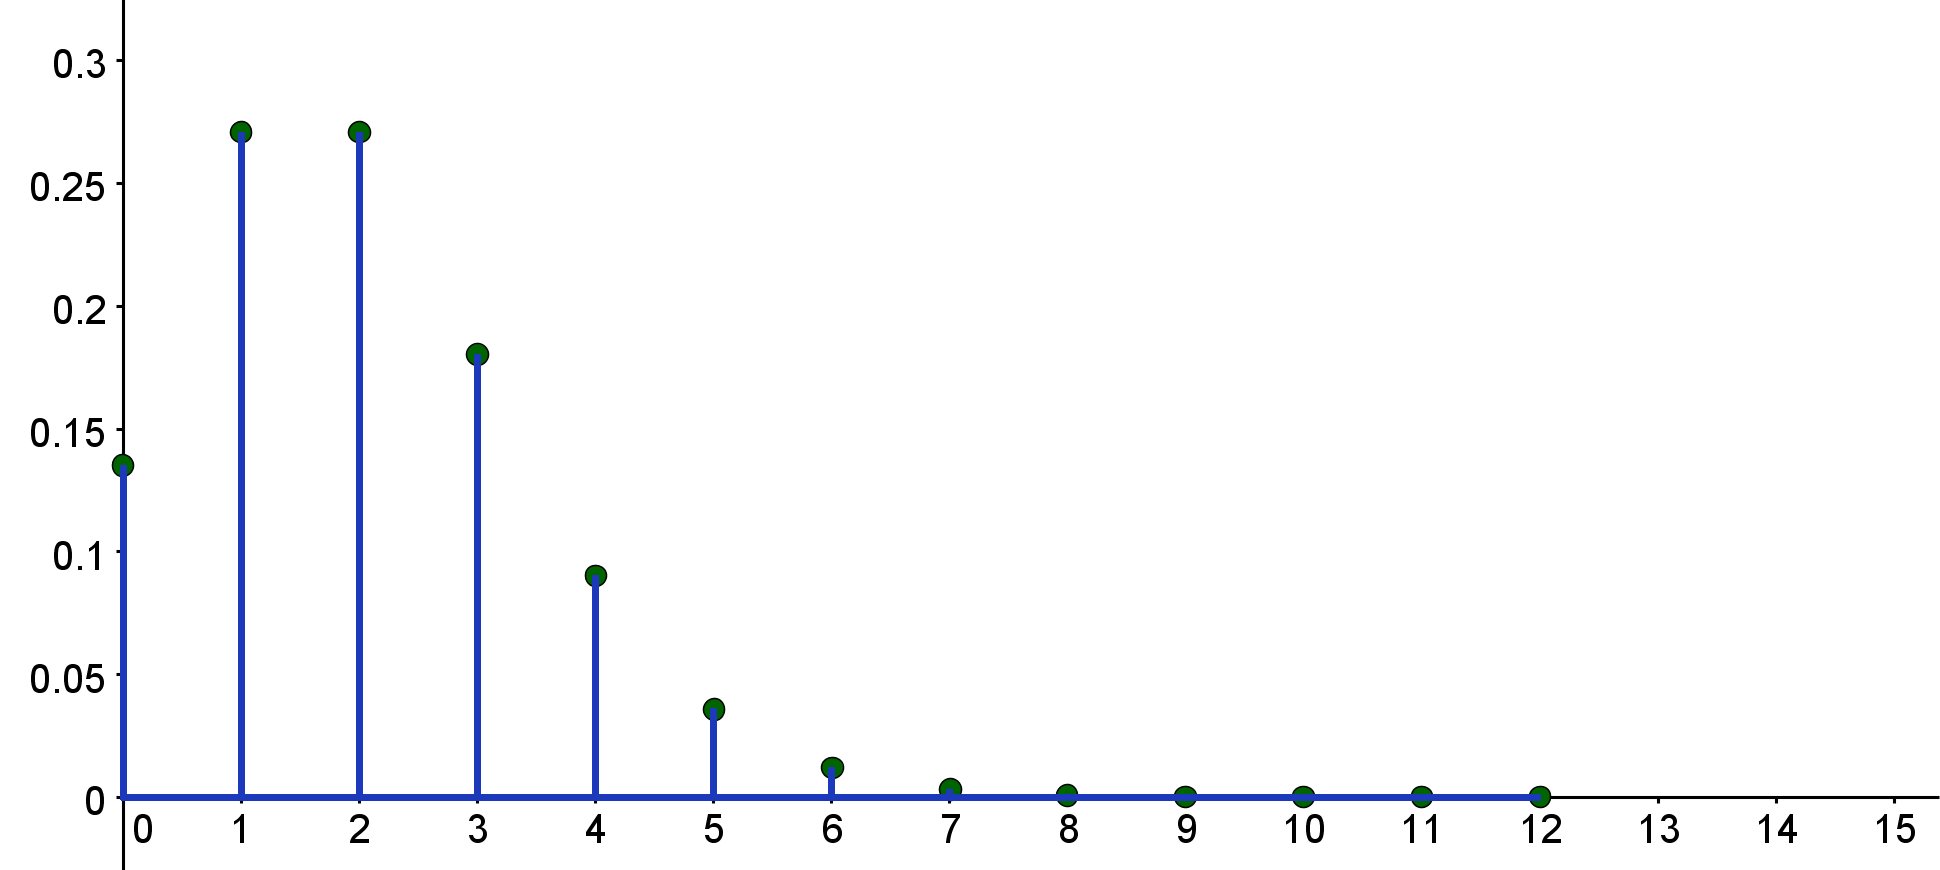
\includegraphics[width=13cm]{../fig/Cap08-PoissonLambda2Probabilidades.png}
\end{enColor}
\begin{bn}
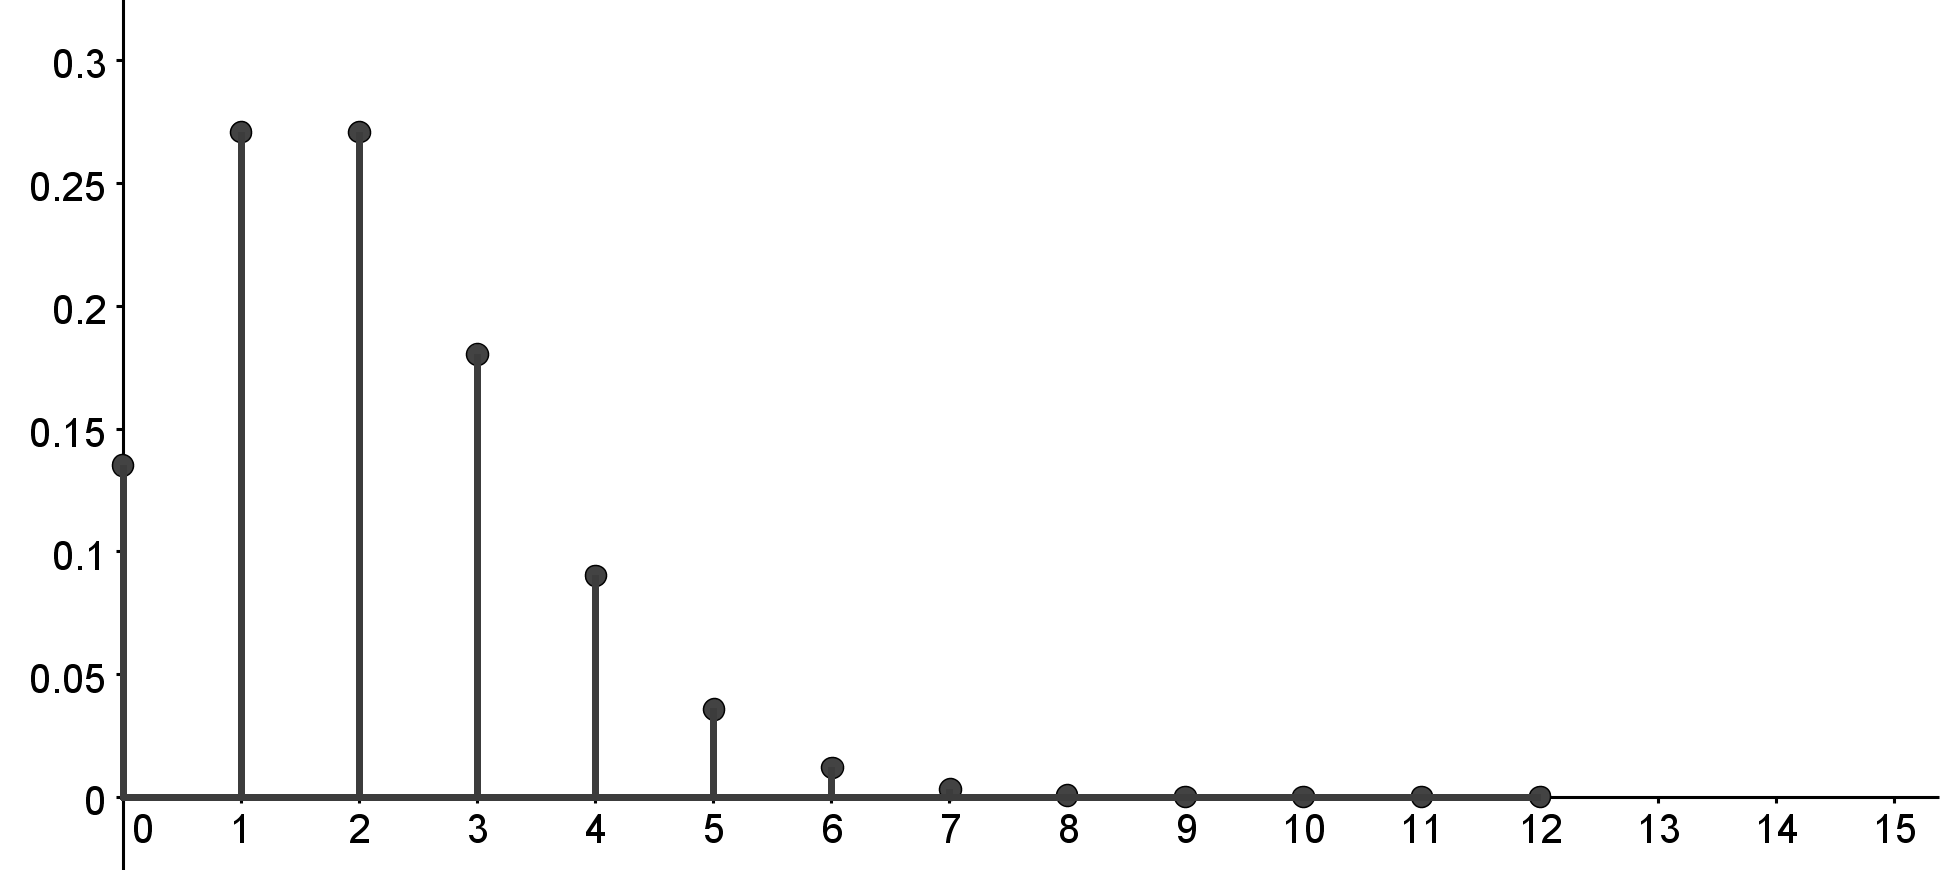
\includegraphics[width=13cm]{../fig/Cap08-PoissonLambda2Probabilidades-bn.png}
\end{bn}
\caption{Valores de probabilidad de la distribución de Poisson con $\lambda=2$. Los valores correspondientes a $k>12$ son muy pequeños, y no se muestran.}
\label{cap07:fig:PoissonLambda2Probabilidades}
\end{center}
\end{figure}

\begin{ejemplo}[{\bf Continuación del Ejemplo \ref{cap08:ejem:PoissonMuertesInfarto01} }]
\label{cap08:ejem:PoissonMuertesInfarto02} En el Ejemplo
\ref{cap08:ejem:PoissonMuertesInfarto01}(pág. \pageref{cap08:ejem:PoissonMuertesInfarto01}) hemos
hecho todos los cálculos suponiendo que la tasa de muertes por infarto en la Comunidad de Madrid
coincide con la media nacional. Y  obtuvimos un valor esperado de 2489 muertes. Manteniendo esa
suposición, vamos a calcular la probabilidad de que el número de muertos por infarto, en 2011, en
la Comunidad de Madrid, sea inferior a 2400 personas. Y lo vamos a hacer de dos maneras, para
ilustrar la aplicación de la distribución de Poisson en problemas como el de este ejemplo.

Por un lado, podemos usar una de las binomiales que aparecieron, a distintos niveles (días, horas,
minutos, etc.), en el Ejemplo \ref{cap08:ejem:PoissonMuertesInfarto01}. Si usamos la binomial
correspondiente al nivel {\em horas}, tendremos $B(n,p)$ con
\[n= \mbox{(nº de horas por año)}\cdot \mbox{(nº de individuos)}=8760 \cdot 6489680,\]
y con $p=p_{hora}\approx 4.379\cdot 10^{-08}$. La probabilidad  que se obtiene (calculada con el ordenador) es
igual a $0.03701$.

Ahora, hagamos la misma cuenta pero usando la distribución de Poisson. ¿Cuál es el valor de
$\lambda$? Naturalmente, debemos usar $2489$, como vimos en el Ejemplo
\ref{cap08:ejem:PoissonMuertesInfarto01}. Y lo que tenemos que calcular, usando una variable $X$ de
tipo $\operatorname{Pois}(\lambda)$, es la probabilidad
\[P(X\leq 2400).\]
En el Tutorial08 aprenderemos a hacer esto usando el ordenador, y veremos que el resultado que se obtiene es exactamente el mismo, $0.03701$, que cuando usamos la anterior binomial.

Naturalmente, cuando usamos el ordenador la diferencia entre ambas formas de llegar al resultado
queda oculta. Pero no debemos perder de vista que, cuando decimos que vamos a usar la binomial en
este ejemplo, estamos hablando de calcular 2400 términos que incluyen cosas como esta:
\[\binom{8760 \cdot 6489680}{2400}\]
Frente a esto, la distribución de Poisson representa un alivio computacional considerable.

No queremos cerrar este ejemplo sin comentar el hecho de que hemos obtenido una probabilidad muy
baja para una cifra de muertes por infarto inferior a 2400 (en 2011 y en Madrid). Pues bien, el INE
informa de que la cifra de muertes por infarto en la Comunidad de Madrid, y en ese año, fue de
1914. En este ejemplo no estamos haciendo, formalmente, un contraste de hipótesis. Pero los
resultados anteriores confirman lo que, en cualquier caso, es un hecho sobradamente conocido: la
tasa de muertes por infarto en la Comunidad de Madrid, por distintas causas, es desde hace años muy
inferior a la media nacional (aprox. un 30\% menor).

\qed
\end{ejemplo}

En la discusión anterior hemos tenido ocasión de ver que el parámetro $\lambda$ coincide con la
media de todas las distribuciones binomiales que usamos para pasar al límite y obtener una variable
Poisson, concretamente de tipo $\operatorname{Pois}(\lambda)$. Así que no debe ser una sorpresa que
la media de una variable $\operatorname{Pois}(\lambda)$ sea, precisamente,  $\lambda$. En lo que se
refiere a la varianza, si se tiene en cuenta que esas binomiales tienen valores de $p$ cada vez más
pequeños (y por lo tanto valores de $q$ cada vez más cercanos a $1$), entonces al recordar las
reflexiones del final de la Sección \ref{cap08:subsec:BinomialesPMuyPequenno}, los siguientes
resultados son los que cabe esperar:
    \begin{center}
    \fcolorbox{black}{Gris025}{
    \begin{minipage}{12.5cm}
        %%%%%%%%%%%%%%%%%%%%%%%%%%%%%%%%%%%%%%%
        \begin{center}
        {\bf Media y varianza de la distribuci\'on de Poisson.}
        \end{center}
       %%%%%%%%%%%%%%%%%%%%%%%%%%%%%%%%%%%%%%%
          Sea $X$ una variable aleatoria discreta de tipo {\sf Poisson $\operatorname{Pois}(\lambda)$}. Entonces su media y varianza vienen dadas por:
          \[\mu_X=\lambda,\qquad \sigma^2_X=\lambda\]
       %%%%%%%%%%%%%%%%%%%%%%%%%%%%%%%%%%%%%%%
    \end{minipage}}
    \end{center}

Naturalmente, para demostrar formalmente esto, es necesario usar la Definición
\ref{cap04:ecu:MediaVariableDiscreta} (pág. \pageref{cap04:ecu:MediaVariableDiscreta}),  teniendo
en cuenta que en este caso se trata de una suma infinita (serie):
    \[\mu_X=\sum_{k=0}^{\infty} k\cdot P(X=k)=
    \sum_{k=0}^{\infty} k\cdot \dfrac{\lambda^k}{k!}e^{-\lambda}\]
    \[=    0\cdot\dfrac{\lambda^0}{0!}e^{-\lambda}+
    1\cdot\dfrac{\lambda^1}{1!}e^{-\lambda}+
    2\cdot\dfrac{\lambda^2}{2!}e^{-\lambda}+\cdots\]
Hay que usar matemáticas algo más complicadas para ver que el valor de esta suma infinita (serie) es $\lambda$. Recomendamos, alternativamente, comprobarlo usando un programa de ordenador (en el Tutorial08 daremos los detalles). El resultado sobre la varianza se
obtiene de una serie similar:
    \[\sigma^2_X=\sum_{k=0}^{\infty} (k-\lambda)^2\cdot P(X=k)=
    \sum_{k=0}^{\infty} (k-\lambda)^2\cdot \dfrac{\lambda^k}{k!}e^{-\lambda}=
    \lambda\]
Esta distribución fue introducida por Siméon Denis Poisson, un físico y matemático francés del siglo XIX, discípulo de Laplace (más información en el enlace [\,\ref{enlace0017}\,]\label{enlace0017a}
de la Wikipedia).

\subsubsection{Aproximación de la binomial por la distribución de Poisson}\label{cap08:subsubsec:AproximacionBinomialPorPoisson}

La forma en que hemos presentado la distribución de Poisson, como límite de la binomial en el caso
de probabilidades pequeñas, permite comprender que podemos usar la distribución de Poisson como
sustituto de la binomial, de forma similar a lo que hicimos con la normal, pero ahora para el caso
de $p$ pequeño. Naturalmente, esa aproximación sólo es válida cuando se cumplen algunas
condiciones. El resultado que vamos a usar este:
    \begin{center}
    \fcolorbox{black}{Gris025}{
    \begin{minipage}{12.5cm}
        %%%%%%%%%%%%%%%%%%%%%%%%%%%%%%%%%%%%%%%
        \begin{center}
        {\bf Aproximación de la binomial por la distribuci\'on de Poisson.}
        \end{center}
       %%%%%%%%%%%%%%%%%%%%%%%%%%%%%%%%%%%%%%%
        Si $X$ es una variable aleatoria discreta de tipo binomial $B(n,p)$ y se cumplen estas dos condiciones:
        \begin{equation}\label{cap08:ecu:CondicionesAproximacionBinomialPorPoisson}
            n\geq 100,\quad \mbox{ y a la vez }\quad p\leq 0.01.
        \end{equation}
        entonces los valores de probabilidad de $X$ se pueden aproximar por los de una distribución de tipo Poisson, concretamente por una $\operatorname{Pois}(\lambda)$, con
        \[\lambda=n\cdot p.\]
       %%%%%%%%%%%%%%%%%%%%%%%%%%%%%%%%%%%%%%%
    \end{minipage}}
    \end{center}

\subsection{Inferencia exacta para la distribución de Poisson.}
\label{cap08:subsec:InferenciaPoisson}

En el caso de la distribución de Poisson, la inferencia de más interés consiste en obtener
intervalos de confianza y realizar contrastes de hipótesis sobre el valor del parámetro $\lambda$.
Pueden encontrarse, en muchos textos, planteamientos basados en el Teorema Central del Límite y la
distribución normal (ver, por ejemplo, \cite{garcia2009estadistica}, pág. 128). Pero, después de nuestro trabajo de la Sección \ref{cap08:subsec:MetodoExactoBinomial} (pág. \pageref{cap08:subsec:MetodoExactoBinomial}), es más interesante, a nuestro juicio, analizar un método de los llamados {\em exactos} para obtener estos intervalos de confianza y contrastes para $\lambda$.

La idea es, por lo tanto, muy parecida a la del método de Clopper y Pearson que hemos descrito en la Sección \ref{cap08:subsec:MetodoExactoBinomial}. Y como allí, vamos a empezar por pensar en contrastes unilaterales, en este caso dirigidos al valor del parámetro $\lambda$ de una distribución de Poisson. Veamos un ejemplo para centrar la discusión.
\begin{ejemplo}
\label{cap08:ejem:ContrasteExactoPoisson}
Supongamos que $X$ es una variable de tipo Poisson. Como ha quedado de manifiesto en el Ejemplo \ref{cap08:ejem:PoissonMuertesInfarto01} (pág. \pageref{cap08:ejem:PoissonMuertesInfarto01}), y en la discusión de esta Sección, el parámetro $\lambda$ se puede interpretar como el número medio de sucesos observados por unidad de tiempo (que puede ser un año, un minuto, etc.; la que se use en el modelo como referencia), en un proceso que reúna las características que hemos descrito. Supongamos que la hipótesis nula sobre $X$ es:
\[H_0=\{ \lambda \leq  7\}\]
y que nosotros hemos observado, en una unidad de tiempo, $11$ apariciones del suceso que medimos (es decir $11$ {\em éxitos}, con terminología binomial). Ese número de sucesos observado, mayor que el valor medio $\lambda_0=7$ que indica la hipótesis nula, nos hace pensar que tal vez sea cierta la hipótesis alternativa:
\[H_a=\{ \lambda > 7\}.\]
{!`}Desde luego, si en lugar de $11$ hubiéramos observado $200$ sucesos, esa sospecha sería casi una certeza, claro! La pregunta que nos hacemos es la pregunta habitual en un contraste: suponiendo que la hipótesis nula es cierta, ¿cuál es la probabilidad de observar un valor como $X=11$, o uno aún más favorable a la hipótesis alternativa? En resumen, ¿cuál es el p-valor para esa observación de $X=11$? En fórmulas:
\[
    \mbox{p-valor}= P(X\geq 11) =\sum_{k=11}^{\infty}P(X=k)=\sum_{k=11}^{\infty}\dfrac{\lambda_0^k}{k!}e^{-\lambda_0}
    =\sum_{k=11}^{\infty}\dfrac{7^k}{k!}e^{-7}
\]
Donde, naturalmente, estamos asumiendo para el cálculo que la hipótesis nula es cierta, y por eso utilizamos el valor $\lambda_0=7$. Esta suma (la cola derecha de la distribución de Poisson) es, con ayuda del ordenador, muy fácil de calcular (como veremos en el Tutorial08), y se obtiene:
\[
    \mbox{p-valor}= P(X\geq 11)\approx 0.09852
\]
Como puede verse, a un nivel del $95\%$ no rechazaríamos la hipótesis nula.
\qed
\end{ejemplo}
La mecánica de los contrastes unilaterales es, como se ve, muy parecida a la que vimos para el caso de las binomiales, por el método de Clopper-Pearson. Y como allí, para el contraste bilateral nos vamos a conformar con la misma receta de cálculo que indicamos en la página \pageref{cap08:ecu:HaBilateralClopperPearson}.

\subsubsection{Intervalos de confianza exactos para $\lambda$}
\label{cap08:subsubsec:IntervaloConfianzaExactoLambdaPoisson}

Y, otra vez, la idea no es nueva. Vamos a aplicar la misma técnica que vimos en la página \pageref{cap08:subsubsec:IntervaloConfianzaExactoPBinomial}. Tenemos un valor observado de $X$, y queremos usarlo para establecer un intervalo de confianza para $\lambda$ a un nivel de confianza, $nc=1-\alpha$ (es decir, que el intervalo debe dejar una probabilidad igual a $\alpha/2$ en cada cola). Lo que hacemos es tomar un valor de $\lambda_0$ para el que {\em no rechazamos} la hipótesis nula
\[H_0=\{ \lambda \leq  \lambda_0\}\]
al nivel de confianza $nc$, y, a continuación, vamos moviendo $\lambda_0$ {\em hacia la izquierda}, hacia valores cada vez menores, hasta encontrar el mayor valor de $\lambda_0$ para el que rechazamos $H_0$. Que será el primer valor para el que obtengamos un p-valor inferior a $\alpha/2$. Ese valor determina el límite inferior del intervalo. Vamos a llamarlo $\lambda_1$. Hacemos lo mismo hacia el otro lado, y localizamos el menor valor de $\lambda_0$ (al que vamos a llamar $\lambda_2$) para el que rechazamos, ahora, la hipótesis nula
\[H_0=\{ \lambda \geq  \lambda_0\}\]
al nivel de confianza $nc$ (de nuevo, buscamos un p-valor inferior a $\alpha/2$). Con eso localizamos el extremo superior del intervalo de confianza buscado, que es el intervalo $(\lambda_1,\lambda_2)$. Veamos un ejemplo concreto.
\begin{ejemplo}{\bf (Continuación del Ejemplo \ref{cap08:ejem:ContrasteExactoPoisson}).}
\label{cap08:ejem:ContrasteExactoPoisson2}
Con el mismo valor observado $X=11$ que hemos encontrado antes, fijamos un nivel de confianza $nc=0.95$ (es decir, $\alpha/2=0.025$). Ahora, empezamos buscando el valor $\lambda_1$ para el que, si $X\sim \operatorname{Pois}(\lambda_1)$, se cumple:
\[
    P(X\geq 11)=0.025
\]
Con ayuda del ordenador, como veremos en el Tutorial08, se obtiene que este valor es, aproximadamente, $\lambda_1\approx 5.491$. De forma análoga, ahora buscamos el valor para el que
si $X\sim \operatorname{Pois}(\lambda_2)$, se cumple:
\[
    P(X\leq 11)=0.025
\]
Ese valor es $\lambda_2\approx 19.68$, y con eso el intervalo de confianza al $95\%$ para $\lambda$ es \[(\lambda_1,\lambda_2)=(5.491,19.68).\]
\qed
\end{ejemplo}



%\pendiente{{\Large TODO LO QUE SE REFIERE A INTERVALOS DE CONFIANZA PARA LA DIS. DE POISSON ME
%PARECE POCO FIABLE. HAY QUE REVISARLO, ANTES DE DECIDIR LO QUE INCLUIMOS. CREO Que lo más sensato
%es incluir algo como lo de la ecuación 6.23, pág. 190 de Rice}}
%
%
%\subsubsection{Aproximación de la distribución de Poisson por una normal}
%\label{cap08:subsubsec:AproximacionPoissonPorNormal}
%
%Al analizar la distribución de Poisson para distintos valores de $\lambda$, se observa que, al
%aumentar $\lambda$, se obtienen distribuciones cada vez más parecidas a la normal. Esto se puede
%considerar como otra manifestación más del Teorema Central del Límite que, en este caso, permite
%aproximar la distribución de Poisson por una normal, siempre que se cumpla una condición sobre
%$\lambda$.
%
%    \begin{center}
%    \fcolorbox{black}{Gris025}{
%    \begin{minipage}{12.5cm}
%        %%%%%%%%%%%%%%%%%%%%%%%%%%%%%%%%%%%%%%%
%        \begin{center}
%        {\bf Aproximaci\'on de la distribuci\'on de Poisson por la normal.}
%        \index{aproximaci\'on de la distribuci\'on de Poisson por la normal}
%        \end{center}
%       %%%%%%%%%%%%%%%%%%%%%%%%%%%%%%%%%%%%%%%
%        Si $X$ es una variable aleatoria discreta de tipo $\operatorname{Pois}(\lambda)$, y se cumple:
%        \[\lambda>5,\]
%        entonces los valores de probabilidad de $X$ se pueden aproximar por los de una distribución de tipo normal, concretamente:
%        \[N(\lambda,\sqrt{\lambda}).\]
%       %%%%%%%%%%%%%%%%%%%%%%%%%%%%%%%%%%%%%%%
%    \end{minipage}}
%    \end{center}
%Un momento: hemos introducido la distribución de Poisson como sustituta de la binomial en algunos
%casos, y ahora ¿sustituimos la distribución de Poisson con una normal? Antes de que el lector se
%pueda sentir más confundido, nos apresuramos a señalar que nuestro objetivo al hacer que la normal
%entre en juego, {\em no es el cálculo de probabilidades}. El cálculo de probabilidades con la
%distribución de Poisson es bastante fácil, y en el Tutorial \pendiente{(FALTA NÚMERO)} veremos como
%usar el ordenador para este fin (adelantamos que, en R, nos van a interesar las funciones {\tt
%ppois} para problemas directos, {\tt qpois} para problemas inversos y {\tt dpois}, para el cálculo
%directo de la función de densidad). La razón por la que ahora interviene la normal es que va a ser
%mucho más fácil de usar, para obtener los intervalos de confianza y contrastes de hipótesis, para
%las variables de tipo Poisson. El esquema, entonces, es este: cuando nos encontramos con una
%variable binomial que cumple las condiciones
%\ref{cap08:ecu:CondicionesAproximacionBinomialPorPoisson} (pág.
%\pageref{cap08:ecu:CondicionesAproximacionBinomialPorPoisson} ), en lugar de utilizar una binomial,
%usamos una distribución de Poisson para describir el fenómeno de que se trate. Y desde luego,
%también en el caso de los procesos de Poisson que hemos descrito antes. Pero, una vez decidido que
%usamos una variable de tipo $Pois(\lambda)$, si queremos construir un intervalo de confianza para
%$\lambda$, o hacer un contraste de hipótesis, lo más sencillo es utilizar las fórmulas que se
%obtienen mediante la aproximación de $Pois(\lambda)$ por una normal. Llevar adelante este plane es
%el último empeño que acometemos en este capítulo.
%
%\subsection{Inferencia para la distribución de Poisson}
%\label{cap08:subsec:InferenciaPoisson}
%
%Debería estar empezando a convertirse en una costumbre: cada nueva distribución que aparece (en este caso la de Poisson) lleva aparejados los correspondientes resultados inferenciales, que se traducen en el cálculo de intervalos de confianza y contrastes de hipótesis. Con la distribución de Poisson, naturalmente, sucede lo mismo. No vamos a considerar el caso de muestras pequeñas, porque sería demasiado complicado. Al limitarnos a muestras grandes, podemos contar con el Teorema Central del Límite, que nos garantiza este resultado:\begin{center}%\\[3mm]
%       \fbox{\colorbox{Gris025}{\begin{minipage}{14cm}
%      \begin{center}
%       %\vspace{2mm}
%       {\bf Teorema central del límite para la distribución de Poisson: }
%      \end{center}
%       Sea $X$ una variable aleatoria de tipo $\operatorname{Pois}(\lambda)$. Si se toman muestras independientes de $X$ de tamaño $n$, entonces cuando $n$ se hace cada vez más grande la distribución de la media muestral
%       $\hat p$ se aproxima cada vez más a la normal $N\left(\lambda,\sqrt{\dfrac{\lambda}{n}}\right)$.\\
%       En particular, para $n$ grande tenemos $Z=\dfrac{\bar X-\lambda}{\sqrt{\dfrac{\mbox{\boldmath $\textcolor{red}{\bar X}$}}{n}}}\sim N(0,1)$.
%       \end{minipage}}}\end{center}%\\[3mm]
%       {\em Obsérvese} que, con vistas a la inferencia, hemos utilizado $\bar X$ como sustituto de $\lambda$ en el cálculo de la desviación típica muestral. Esta sustitución es similar a otras que ya hemos encontrado.
%
%Como en el caso de las proporciones, tras establecer la distribución de la media muestral, es inmediato obtener el intervalo de confianza:\begin{center}%\\[3mm]
%       \fbox{\colorbox{Gris025}{\begin{minipage}{14cm}
%       \begin{center}
%       %\vspace{2mm}
%       {\bf Intervalo de confianza (nivel $(1-\alpha$)) para $\lambda$ (en $\operatorname{Pois}(\lambda)$), con muestra grande: }
%       \index{\bf Intervalo de confianza para $\lambda$ (en $\operatorname{Pois}(\lambda)$)}
%       \end{center}
%       Si consideramos muestras de tamaño $n$ suficientemente grandes, entonces el intervalo de confianza al nivel $(1-\alpha)$  para $\lambda$  es:
%       \[\bar X-z_{\alpha/2}\sqrt{\dfrac{\bar X }{n}}\leq \lambda \leq \bar X +z_{\alpha/2}\sqrt{\dfrac{\bar X}{n}}.\]
%       que también escribiremos $\lambda =\bar X \pm z_{\alpha/2}\sqrt{\dfrac{\bar X}{n}}$.
%       \end{minipage}}}\end{center}%\\[3mm]
%       Y los contrastes de hipótesis unilaterales y bilaterales {\em ({!`}de nuevo, hay que prestar atención a los valores de $z$ utilizados en cada caso!)}:
%       \begin{center}%\\[3mm]
%       \fbox{\colorbox{Gris025}{\begin{minipage}{14cm}
%      \begin{center}
%%       \vspace{2mm}
%       {\bf Contraste de hipótesis (nivel $(1-\alpha$)) para $\lambda$ (en $\operatorname{Pois}(\lambda)$), con muestra grande: }\index{contraste de hipótesis para $\lambda$  (en $\operatorname{Pois}(\lambda)$)}
%      \end{center}
%       Si consideramos muestras de tamaño $n$ suficientemente grandes, entonces se tienen los siguientes contrastes de hipótesis:
%       \begin{enumerate}
%       \item[(a)] Hipótesis nula: $H_0=\{\lambda\leq \lambda_0\}$.\\
%            Región de rechazo $\bar X>\lambda_0+z_{\alpha}\sqrt{\dfrac{\lambda_0}{n}}.$
%       \item[(b)] Hipótesis nula: $H_0=\{\lambda\geq \lambda_0\}$.\\
%            Región de rechazo: $\bar X<\lambda_0+z_{1-\alpha}\sqrt{\dfrac{\lambda_0}{n}}.$
%       \item[(a)] Hipótesis nula: $H_0=\{\lambda=\lambda_0\}$.\\
%            Región de rechazo: $|\bar X-\lambda_0|>z_{\alpha/2}\sqrt{\dfrac{\lambda_0}{n}}.$
%       \end{enumerate}
%       \end{minipage}}}
%       \end{center}%\\[3mm]
%       Una observación, muy parecida a la que hicimos en el caso de los contrastes sobre proporciones. Puesto que el contraste se basa en suponer que la hipótesis nula es cierta, hemos utilizado $\lambda_0$ en lugar de $\bar X$. Y de nuevo, la razón de hacer esto es que, como hemos dicho, si suponemos que la hipótesis nula es cierta, entonces la desviación típica de la media muestral sería $\sqrt{\dfrac{\lambda_0}{n}}$.
